\section{Abstract}
This Chapter presents a search for exotic decays of the Higgs boson to a pair of new (pseudo)scalar
particles, $H\to aa$, with a mass in the range 20--60 \GeV{}, and where one of the $a$ bosons decays into a pair of photons and the other to a pair of gluons.
The results of this search are published in~\cite{Aaboud:2018gmx}.
The search is performed in event samples enhanced in vector-boson fusion Higgs boson production
by requiring two jets with large invariant mass in addition to the Higgs boson candidate decay products.
The analysis is based on the full dataset of $pp$ collisions at $\sqrt{s}= 13$ \TeV{} recorded in 2015 and 2016 with the ATLAS detector at the CERN Large Hadron Collider,
corresponding to an integrated luminosity of 36.7 \ifb.
The data are in agreement with the Standard Model predictions and an upper limit at the 95\% confidence level is placed on the production cross section times the
branching ratio for the decay $H\to aa\to \gamma\gamma gg$.
This limit ranges from 3.1 pb to 9.0 pb depending on the mass of the $a$ boson.


\section{Introduction}

The search for the Standard Model (SM) Higgs 
boson~\cite{Englert:1964et,Higgs:1964pj,Higgs:1964ia,Guralnik:1964eu}  
has been one of the main goals of the LHC physics program.  
A new particle with mass  of 125 GeV, and with  properties compatible with those expected for the SM Higgs boson, 
has been discovered by the ATLAS~\cite{HIGG-2012-27} and CMS~\cite{CMS-HIG-12-028} collaborations.
Since its discovery, a comprehensive program of measurements of the properties of this particle has been underway.
These measurements could uncover deviations from expected SM branching ratios or 
allow for the possibility of decays into new particles. 

Existing measurements constrain the branching ratio for such decays ($\text{B}_\text{exotic}$) 
to less than 34\% at 95\% confidence level~\cite{Khachatryan:2016vau}.
Exotic decays are predicted by many theories of physics beyond the SM~\cite{Curtin:2013fra},
including those with an extended Higgs sector 
such as the Next-to-Minimal Supersymmetric Standard Model 
~\cite{Dobrescu:2000yn,Ellwanger:2003jt,Dermisek:2005ar,Chang:2008cw,Morrissey:2008gm},
several models of dark matter~\cite{SILVEIRA1985136,Pospelov:2007mp,Draper:2010ew,Ipek:2014gua,Martin:2014sxa},
models with a first order electroweak phase transition~\cite{Profumo:2007wc,Blinov:2015sna},
and theories with neutral naturalness~\cite{Burdman:2006tz,Craig:2015pha,Curtin:2015fna}.
These theories are motivated by some of the most outstanding unanswered questions in physics, such as the gauge hierarchy problem~\cite{Nilles:1982dy}, the nature of dark matter~\cite{Trimble:1987ee}, and the strong CP problem~\cite{Peccei:1977hh}.

One of the simplest possibilities is that the Higgs boson decays to a pair of 
new scalars or pseudoscalars, $a$, which in turn decay to a pair of SM particles.
Several searches have been performed for $H\rightarrow a a$ in various final states~\cite{Khachatryan:2017mnf,Aad:2015sva,Aad:2015oqa}.

The work presented here explores in particular the search for $H\rightarrow a a$, where the final state contains two photons ($\gamma$) and two gluons ($g$) ($H\rightarrow aa \rightarrow \gamma\gamma gg$).
This decay mode becomes relevant in models where the $a\rightarrow$ fermion decays are suppressed 
and the $a$ decays only to photons and gluons
~\cite{Curtin:2013fra,hep-ph/0703247}.
The ATLAS Run 1 search for $H\rightarrow aa \to 4\gamma$~\cite{Aad:2015bua} sets 
a limit $\sigma\times \text{B}(H\to aa\rightarrow 4\gamma)<10^{-3}\sigma_\text{SM}$ 
for $10~\GeV<m_a<62~\GeV$.
Before this work, there was no direct limit set on $\text{B}(H\rightarrow aa\rightarrow \gamma\gamma gg)$;
however, in combination with $\text{B}_\text{exotic}<34\%$, 
the $H\rightarrow 2a \to 4\gamma$ result sets indirect limits on $\text{B}(H\rightarrow aa\rightarrow \gamma\gamma gg)$ to less than $\sim4\%$ (Appendix~\ref{sec:HBSM_app:existinglimits}).
Assuming a SM-like ratio of photon and gluon couplings, 
the $H\rightarrow 4\gamma$ decay occurs very rarely relative to the $H\rightarrow \gamma\gamma gg$ decay (a typical value of the relative ratio of branching ratios is $3.8\times10^{-3}$~\cite{hep-ph/0703247})
\footnote{The $H\rightarrow 4g$ final state is the most common, but is unfortunately swamped by background.},
making the $H\rightarrow \gamma\gamma gg$ an excellent unexplored final state for probing these fermion-suppressed models.
The branching ratio for $a\rightarrow \gamma\gamma$ can be enhanced in some scenarios;
the two searches are therefore complementary, 
where the $H\rightarrow \gamma\gamma gg$ final state is more sensitive to SM-like photon couplings 
with the new physics sector, 
while the $H\rightarrow 4\gamma$ final state is more sensitive to the enhanced photon scenarios. 

The most common Higgs production modes at the LHC are through gluon fusion (ggF), vector boson fusion (VBF), or associated production with an additional vector boson (VH)~\cite{Dittmaier:2011ti}.
The cross sections for each of these Higgs production modes is in a ratio of roughly 100:10:1~\cite{deFlorian:2016spz}; targeting any individual production mode requires a tradeoff between higher production cross section and increased handles on distinguishing signal from background.
Ref.~\cite{hep-ph/0703247} shows that the search for $H \to \gamma\gamma gg$ in the VH mode, 
where the additional vector boson
decays leptonically, would require approximately $300~\ifb$ of LHC data in order to be sensitive to branching ratios less than 4\%. 
While the gluon fusion production has a larger cross section, it is overwhelmed by background.
We have found (Figure~\ref{fig:HBSM:HBSM_prodmodes}) that the search in the VBF production 
mode can achieve sensitivity competitive with or better than the above two production modes in the range $20$ to $300~\ifb$ of LHC integrated luminosity data,
and in particular with the approximately $150~\ifb$ of data at the end of LHC Run 2~\cite{lhc-commissioning}.

In the VBF production mode, two extra quarks are produced along with the Higgs in the hard scatter interaction.
The gluons from the Higgs decay and the quarks from the VBF production are reconstructed as jets ($j$) in the ATLAS detector;
therefore, this search is focused on the $H\to2\gamma2j$ final state with two additional jets from the VBF production.
Figure~\ref{fig:HBSM:VBFH_feynman} shows a tree-level Feynman diagram of the VBF production and $\gamma\gamma gg$ decay of the Higgs boson, including the $aa$ intermediate state.

\begin{figure}[t]
  \centering 
  \subfloat[]{\includegraphics[width=0.45\textwidth]{figures/{HBSM_prodmodes}.pdf}\label{fig:HBSM:HBSM_prodmodes}}
  \subfloat[]{
    \begin{tikzpicture}
      \begin{feynman}
        \vertex (q1init) {\(q\)};
        \vertex [below =4. of q1init] (q2init) {\(q\)};
        \vertex [below right=1. and 2. of q1init] (qqV);
        \vertex [above right=1. and 2. of q2init] (qqV2);
        \vertex [above right=1. and 4. of  qqV] (q1final) {\(q\)};
        \vertex [below right=1. and 4. of qqV2] (q2final) {\(q\)};
        \vertex [below right=1. and 1. of qqV] (VVH);
        \vertex [right=1. of VVH] (H);
        \vertex [above right=1. and 1. of H] (ayy);
        \vertex [below right=1. and 1. of H] (agg);
        \vertex [above right=0.5 and 1. of ayy] (y1) {\(\gamma\)};
        \vertex [below right=0.5 and 1. of ayy] (y2) {\(\gamma\)};
        \vertex [above right=0.5 and 1. of agg] (g1) {\(g\)};
        \vertex [below right=0.5 and 1. of agg] (g2) {\(g\)};
        \diagram* {
          (q1init) -- [fermion] (qqV) -- [fermion] (q1final),
          (q2init) -- [fermion] (qqV2) -- [fermion] (q2final),
          (qqV) -- [boson, edge label'=\(V\)] (VVH),
          (qqV2) -- [boson, edge label'=\(V\)] (VVH),
          (VVH) -- [scalar, edge label'=\(H\)] (H),
          (H) -- [scalar, edge label'=\(a\)] (ayy),
          (H) -- [scalar, edge label'=\(a\)] (agg),
          (ayy) -- [photon] (y1),
          (ayy) -- [photon] (y2),
          (agg) -- [gluon] (g1),
          (agg) -- [gluon] (g2),
        };
      \end{feynman}
    \end{tikzpicture}
    \label{fig:HBSM:VBFH_feynman}
  }
  \caption{
    (a) Projected branching ratio for $H\rightarrow \gamma\gamma gg$ in order to make a discovery of new physics at a significance level of $5\sigma$, as a function of integrated luminosity, when searching in the gluon fusion (GGH), vector boson fusion (VBF), and associated production (VH) production modes.
    The projection for GGH and VBF assumes a $20\%$ systematic uncertainty due to jet reconstruction effects, while the projection for VH uses the estimation from~\cite{hep-ph/0703247}, assuming the significance is statistics-dominated.
    With less than $\sim 20 \ifb$, the gluon fusion mode is most sensitive, but with more statistics this production mode quickly becomes dominated by systematic uncertainties and is unable to provide better limits.
    Up to $\sim 300 \ifb$, the VBF mode is most sensitive; in Run 2 the LHC has gathered 140$\ifb$.
    With more than $\sim 300 \ifb$, the VH mode likely provides the best sensitivity.
    (b) Tree-level diagram of production and decay of Higgs boson being searched for in this analysis.
    }
\end{figure}

\clearpage
\section{Data and simulation}
The search presented in this chapter is based on the 36.7~\ifb{} dataset of proton--proton collisions
recorded by the ATLAS experiment at the LHC at $\sqrt{s}=13$ \TeV{} during 2015 and 2016.
As discussed in Chapter~\ref{ch:ATLAS}, the ATLAS detector~\cite{PERF-2007-01} comprises an inner detector in a 2 T axial magnetic field, 
for tracking charged particles and a precise localisation of the interaction vertex, 
a finely segmented calorimeter, a muon spectrometer and a two-level trigger~\cite{TRIG-2016-01} that
accepts about 1 kHz rate for data storage.

Monte Carlo (MC) event generators were used to simulate the $H\to aa \to \gamma\gamma gg$ signal.
Signal samples for the ggF and VBF processes were generated at next-to-leading order using 
\POWHEGBOX{}~\cite{Nason:2004rx,Frixione:2007vw,Alioli:2010xd} interfaced with \PYTHIA{}~\cite{Sjostrand:2014zea} for parton showering and hadronisation using the AZNLO set of tuned parameters set~\cite{STDM-2012-23} and the CT10 parton distribution function (PDF) set~\cite{Lai:2010vv}.
Samples were generated in the $m_a$ range\footnote{The diphoton triggers considered for this
search do not have acceptance for the lower mass range ($m_a<20~\GeV{}$), where the two photons are collimated.} 
$20~\GeV{} < m_a < 60~\GeV{}$, assuming the $a$ boson to be a (pseudo)scalar.
All MC event samples were processed through a detailed simulation~\cite{SOFT-2010-01} of the ATLAS detector
based on \geantFour{}~\cite{Agostinelli:2002hh}, and contributions from additional $pp$ interactions (pile-up), simulated using
\PYTHIA{} and the MSTW2008LO PDF set~\cite{Martin:2009iq}, were overlaid onto the hard-scatter events.

\section{Event Selection}
\subsection{Trigger}
\label{sec:HBSM:trigger}
Events are selected by requiring at least one of two diphoton triggers.
One trigger path requires the presence in the electromagnetic (EM) calorimeter of two clusters of energy
deposits with transverse energy
%\footnote{ATLAS uses a right-handed coordinate system with its origin at the nominal interaction point (IP) in the centre of the detector and the $z$-axis along the beam pipe. The $x$-axis points from the IP to the centre of the LHC ring, and the $y$-axis points upward. Cylindrical coordinates $(r,\phi)$ are used in the transverse plane, $\phi$ being the azimuthal angle around the $z$-axis. The pseudorapidity is defined in terms of the polar angle $\theta$ as $\eta=-\ln\tan(\theta/2)$.}
above 35 \GeV{} and 25 \GeV{} for the leading (highest transverse energy) and sub-leading
(second-highest transverse energy) clusters, respectively.
In the high-level trigger the shape of the energy deposit in both clusters is required to be loosely consistent with that expected from an EM shower initiated by a photon.
The other trigger path requires the presence of two clusters with transverse energy above 22 \GeV{}.
In order to suppress the additional rate due to the lower transverse energy threshold, the shape requirements for the energy deposits are
more stringent.
Using the ATLAS trigger nomenclature, these two trigger paths are called \texttt{HLT\_g35\_loose\_g25\_loose} and \texttt{HLT\_2g22\_tight}, respectively.
Both of these high-level trigger are seeded by the Level 1 trigger \texttt{L1\_2EM15VH}, which requires two Level 1 objects consistent with the EM shower initiated by a photon with transverse energy greater than $15$ \GeV{}.
In 2015 and 2016 data these triggers were unprescaled.
The efficiency of each of the triggers on signal events with $m_a=30$ \GeV{} is shown in Table~\ref{tab:HBSM:trigeff}.
The efficiency of requiring at least one of the two triggers for other masses of $m_a$ can be seen in Figure~\ref{fig:HBSM:cutflow_ma}.
The trigger efficiency notably goes down for $m_a<20$ \GeV{}; this limits the sensitivity of this search.
The cause of this trigger inefficiency is discussed in Appendix~\ref{sec:HBSM_app:lowmass}.

\begin{table}[]
\centering
  \caption{Efficiency of triggers on a signal sample with $m_a=30$ GeV. The efficiencies are shown for the signal MC separated by production in the VBF and GGF modes, and for the combined production modes.}
\label{tab:HBSM:trigeff}
\begin{tabular}{|l|l|l|l|l|l|}
\hline
                                                      & \multicolumn{3}{c|}{Efficiency}  \\ \hline
                                                      & VBF      & ggF  & Combined   \\ \hline
\texttt{HLT\_g35\_loose\_g25\_loose}                  & 0.158  & 0.161 & 0.160\\ \hline
\texttt{HLT\_2g22\_tight}                             & 0.166  & 0.208 & 0.200\\ \hline
OR of triggers                                        & 0.201  & 0.242 & 0.234\\ \hline
\end{tabular}
\end{table}

\subsection{Photons}
\label{sec:HBSM:photons}
The photon candidates are reconstructed from the clusters of energy deposits in the EM calorimeter within the range $|\eta|<2.37$.
The energies of the clusters are calibrated to account for energy losses upstream of the calorimeter and for energy leakage outside the cluster, as well as other effects due to the detector geometry and response.
The calibration is refined by applying $\eta$-dependent correction factors of the order of $\pm1$\%, derived from $Z\to ee$ events~\cite{PERF-2013-05}.
As in the trigger selection, photon candidates are required to satisfy a set of identification criteria based on the shape of the EM cluster~\cite{PERF-2013-04}.
Two working points are defined: a \textit{Loose} working point, used for the preselection and the data-driven background estimation, and a 
\textit{Tight} working point, with requirements that further reduce the misidentification of neutral hadrons decaying to two photons.
In order to reject the hadronic jet background, photon candidates are required to be isolated from any other activity in the calorimeter.
The calorimeter isolation is defined as the sum of the transverse energy in the
calorimeter within a cone of \mbox{$\Delta R = \sqrt{(\Delta\eta)^2+(\Delta\phi)^2}=0.4$} centered around the photon candidate,
The transverse energy of the photon candidate is subtracted from the calorimeter isolation.
Contributions to the calorimeter isolation from the underlying event and pile-up are subtracted using the method proposed in~\cite{Cacciari:2007fd}.
Candidates with a calorimeter isolation larger than 2.2\% of the photon's transverse energy are rejected.

Events are required to have at least two photon candidates. 
The transverse energy requirements depend on the trigger path through which the event was recorded.
For events passing the trigger with higher transverse energy thresholds (\texttt{HLT\_g35\_loose\_g25\_loose}), the leading photon is required to have $E_\text{T}>40$ \GeV{}, and the sub-leading photon is required to have $E_\text{T}>30$ \GeV{}.
For events passing the trigger with lower thresholds (\texttt{HLT\_2g22\_tight}), both the leading and sub-leading photons are required to have $E_\text{T}>27$ \GeV{}. 
For events passing both triggers, the latter selection is applied.

The efficiency of requiring at least two photon candidates in the signal can be seen in Figure~\ref{fig:HBSM:cutflow_ma}.
This photon selection efficiency notably goes down for $m_a<20$ \GeV{} (beyond the inefficiency from the diphoton trigger); this further limits the sensitivity of this search.
The cause of this inefficiency is discussed in Appendix~\ref{sec:HBSM_app:lowmass}, but is mostly due to the calorimeter isolation on photons discussed above.

The invariant mass of the two leading photon candidates is denoted by $m_{\gamma\gamma}$.
The $m_{\gamma\gamma}$ resolution is excellent, with $>\sim97\%$ of signal events satisfying $|m_{\gamma\gamma}-m_a|<2.5$ \GeV{}, regardless of the value of $m_a$; this can be seen in Figure~\ref{fig:HBSM:photon_kinematics}.

\begin{figure}[htbp]
  \centering 
  \subfloat[]{\includegraphics[width=0.45\textwidth]{figures/{myy_unscaled_combine_ma_VBF8_8.7.17_public}.pdf}}
  \subfloat[]{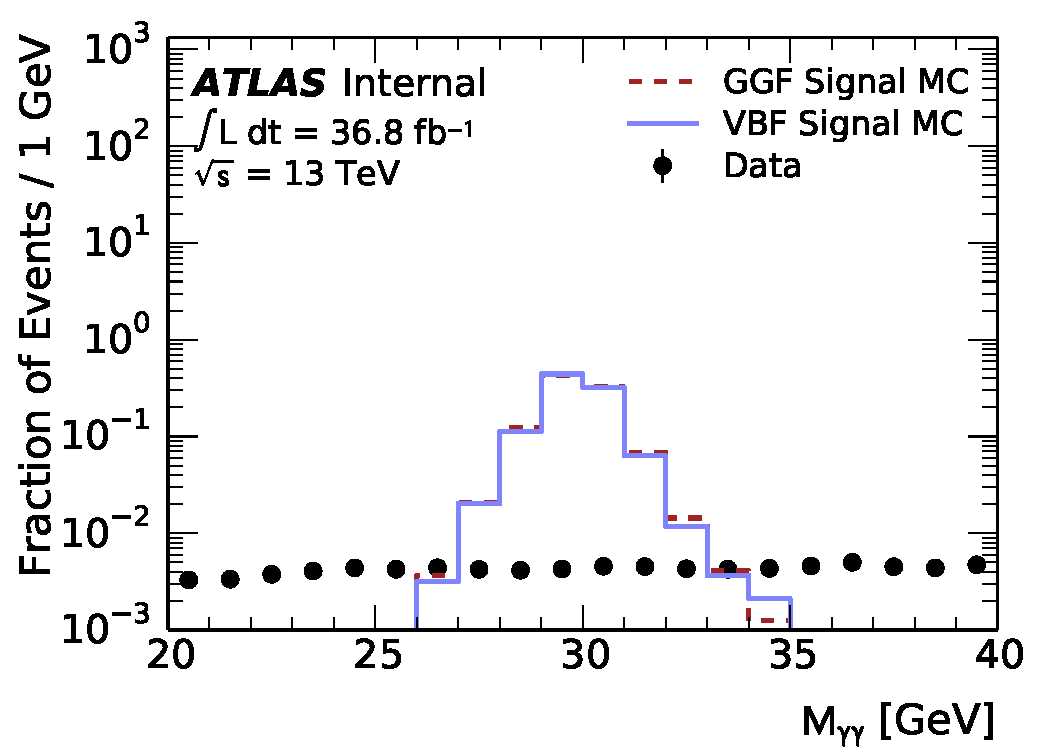
\includegraphics[width=0.45\textwidth]{figures/myy_shape_log.pdf}}\\
  \caption{Distribution of $m_{\gamma\gamma}$. The quantities are plotted separately for signal MC produced in the VBF and GGF modes. (a) The distribution for some of the signal samples used in this analysis (each signal normalized to a branching ratio BR($H\rightarrow aa \rightarrow \gamma\gamma jj)=0.03$). (b) Zoomed in distribution, for a signal with $m_a=30$ GeV.}
  \label{fig:HBSM:photon_kinematics}
\end{figure}

\subsection{Jets}
\label{sec:HBSM:jets}
Jets are reconstructed from topological clusters~\cite{Aad:2016upy} using the anti-$k_t$
algorithm~\cite{Cacciari:2008gp} implemented in the FastJet package~\cite{Cacciari:2011ma} with a radius parameter of $R=0.4$. 
Jets are calibrated using an energy- and $\eta$-dependent
calibration scheme, and are required to have a transverse momentum (\pt{}) greater than $20~\GeV{}$ and $|\eta|<2.5$ or $\pt>30~\GeV{}$ and $|\eta|<4.4$.
The jets with $|\eta|<2.5$ are referred to as \textit{central} jets and those with $2.5<|\eta|<4.4$ are referred to as \textit{forward} jets.
In this analysis both central and forward jets are used, however the requirements on these two categories of jets differ due to the treatment of pile-up jets in the central and forward region of the detector.
Central jets with $p_T<60$ GeV and $|\eta|$<2.4 are required to satisfy the \textit{Default} Jet Vertex Tagger selection~\cite{Aad:2015ina}.
Forward jets with $p_T<50$ GeV are required to pass the \textit{Tight} forward JVT cut~\cite{Aaboud:2017pou}. 
Jets must have an angular separation of $\Delta R>0.4$ from any \textit{Loose} photon candidate in the event.

In the VBF production mode, the Higgs boson is produced in association with two additional light-quark jets
with a large opening angle and a large invariant mass.
Selected events are therefore required to have at least four jets.

\subsection{Preselection}
The preselection detailed in Sections~\ref{sec:HBSM:trigger},~\ref{sec:HBSM:photons}, and~\ref{sec:HBSM:jets} is summarized in Table~\ref{tab:HBSM:preselection}.

\begin{table}[htbp]
  \begin{center}
  \caption{Event preselection.}
  \label{tab:HBSM:preselection}
    {\footnotesize
  \begin{tabular}{ l c c}
    \toprule
    & \multicolumn{2}{c}{Selection} \\
    \midrule
    L1 trigger  & \multicolumn{2}{c}{\texttt{L1\_2EM15VH}} \\
    \\
    Primary HLT trigger  & \texttt{HLT\_g35\_loose\_g25\_loose} & \texttt{HLT\_2g22\_tight} \\
    \\ 
%    \multirow{2}{*}{Photon Selection} & $\geq 1$ photon with $E_T>35$ \GeV{} and $|\eta|<2.5$ \\
%                                      & $\geq 2$ photons with $E_T>25$ \GeV{} and $|\eta|<2.5$\\ 
%    \\
%    \multirow{4}{*}{Jet Selection} & $\geq 4$ jets with: \\
%                                   & $p_T>20$ \GeV{} and $|\eta|<2.5$ \\
%                                   & or \\
%                                   & $p_T>30$ \GeV{} and $2.5<|\eta|<4.5$\\ 
    \multirow{2}{*}{Photon Selection} & $\geq 2$ photons with $E_\text{T}>30$ \GeV{} & $\geq 2$ photons with $E_\text{T}>27$ \GeV{}\\ 
                                      & $\geq 1$ photon with $E_\text{T}>40$ \GeV{}\\
    \\
    Jet Selection & \multicolumn{2}{c}{$\geq 4$ jets, central or forward} \\
    \\
    \bottomrule
  \end{tabular}
    }
  \end{center}
\end{table}

After the preselection, the expected dominant contribution to the background consists of events with two real radiated photons and additional radiated jets (photons + jets), as well as events with multiple jets with one or two of those falsely passing the photon identification requirements (fake photon + jets).
Ultimately the background estimation is entirely data-driven, but the remaining selections are intended to enhance the signal presence while reducing the presence of this background component.

\subsection{VBF Selection}
\label{sec:HBSM:VBF_sel}
The two additional light-quark jets that are produced in association with the Higgs boson in the VBF production mode tend to have a large opening angle and therefore a large combined invariant mass.
The pair of jets with the highest invariant mass ($m_{jj}^\text{VBF}$, or VBF $m_{jj}$) are referred to as \textit{VBF jets}.
The two remaining highest-\pt{} jets are referred to as \textit{signal jets}, with invariant mass $m_{jj}$.
The jet assignment is designed to choose the correct VBF and signal jets for VBF signal events. The truth parton label (the truth ID of the highest $p_T$ parton in the jet) is used to study the accuracy of this jet assignment in MC.

As seen in Figure~\ref{fig:numIDjets}, after the 4 jet preselection requirement, about 70\% of VBF signal events contain at least 2 gluon jets; also, about 70\% of VBF signal events contain at least 2 quark jets. This limits the possible accuracy of the jet assignment.

\begin{figure}[htbp]
  \centering 
  \subfloat[]{\includegraphics[width=0.45\textwidth]{figures/{VBF7_numgluonjets_4j_VBF_a30_ggyy_6.21.17_Nominal}.pdf}}
  \subfloat[]{\includegraphics[width=0.45\textwidth]{figures/{VBF7_numquarkjets_4j_VBF_a30_ggyy_6.21.17_Nominal}.pdf}}
  \caption{Jet multiplicity of (a) gluon and (b) quark jets in a VBF signal sample with $m_a=30$ GeV.}
  \label{fig:numIDjets}
\end{figure}

The best possible jet assignment would choose the two gluon jets with mass closest to $m_a$ as the signal jets and two quark jets as the VBF jets, if such an assignment is possible.
Figure~\ref{fig:truegluon} shows the results of this assignment (which can only be done at truth level) for a VBF signal sample with $m_a=30$ GeV.

In the $m_{jj}$ distribution there is a peak about $m_a$ with width about $0.4m_a = 12$ GeV.
Only about 35\% of the events have two gluons with an invariant mass within this peak; this indicates that most of the time the two true signal gluons are either not reconstructed or below the jet $p_T$ cut.
This 12 GeV width also informs the choice of a $0.4m_a$ cut on $|m_{jj}-m_{\gamma\gamma}|$ in the ABCD regions definition (\ref{sec:HBSM:signal_selection}).

\begin{figure}[htbp]
  \centering 
  \subfloat[]{\includegraphics[width=0.45\textwidth]{figures/{VBF7_count_ids_bar_true_gluon_signal_VBF_a30_ggyy_6.21.17_Nominal}.pdf}}
  \subfloat[]{\includegraphics[width=0.45\textwidth]{figures/{VBF7_mjj_true_gluon_signal_VBF_a30_ggyy_6.21.17_Nominal}.pdf}}
  \caption{(a) Truth parton label of jets chosen as signal jets in a VBF signal sample with $m_a=30$ GeV; the jet assignment is to choose the two truth gluons with mass closest to $m_a$ as the signal jets and the two highest $p_T$ truth quark jets as the VBF jets, if such an assignment is possible (i.e., this assignment can only be done at truth level). (b) The distribution of $m_{jj}$ for the signal jets.}
  \label{fig:truegluon}
\end{figure}

Figure~\ref{fig:remove} shows the results of the jet assignment used in this analysis for a VBF signal sample with $m_a=30$ GeV.
About 20\% of the events choose two gluons with an invariant mass within 12 GeV of $m_a$ as the signal jets.
About 55\% of the events choose two quarks correctly as the VBF jets.

Figure~\ref{fig:VBFmjj_quarkquark} examines the distribution of VBF $m_{jj}$ with the jet assignment used in this analysis in a VBF signal sample with $m_a=30$ GeV using truth information.
The distributions are compared among all events, events where both VBF jets are truth identified as quarks, and events where at least one VBF jet is not truth identified as a quark.
It can be seen that the VBF $m_{jj}$ distribution is shifted upwards relative to the case where the truth quarks are not correctly selected, but the case where the truth quarks are always correctly selected is shifted to even higher values.

Figure~\ref{fig:remove} also shows the results of the jet assignment used in this analysis for a gluon fusion signal sample with $m_a=30$ GeV and for a photons + jets background MC sample.
In the gluon fusion signal sample, about 20\% of the events choose two gluons with an invariant mass within 12 GeV of $m_a$ as the signal jets.
In these events the jets labeled the ``VBF jets'' in fact come from pileup, underlying event, or initial or final state radiation. 

\begin{figure}[htbp]
  \centering 
  \subfloat[]{\includegraphics[width=0.45\textwidth]{figures/{VBF7_count_ids_bar_remove_VBF_a30_ggyy_6.21.17_Nominal}.pdf}}
  \subfloat[]{\includegraphics[width=0.45\textwidth]{figures/{VBF7_count_ids_bar_remove_VBFID_VBF_a30_ggyy_6.21.17_Nominal}.pdf}}\\
  \subfloat[]{\includegraphics[width=0.45\textwidth]{figures/{VBF7_count_ids_bar_remove_ggH_a30_ggyy_6.21.17_Nominal}.pdf}}
  \subfloat[]{\includegraphics[width=0.45\textwidth]{figures/{VBF7_count_ids_bar_remove_VBFID_ggH_a30_ggyy_6.21.17_Nominal}.pdf}}\\
  \subfloat[]{\includegraphics[width=0.45\textwidth]{figures/{VBF7_count_ids_bar_remove_myy_0_55_7.6.17_Nominal}.pdf}}
  \subfloat[]{\includegraphics[width=0.45\textwidth]{figures/{VBF7_count_ids_bar_remove_VBFID_myy_0_55_7.6.17_Nominal}.pdf}}\\
  \caption{Truth parton label of jets chosen as (a) signal jets and (b) VBF jets in a VBF signal sample with $m_a=30$ GeV; (c) signal jets and (d) VBF jets in a gluon fusion signal sample with $m_a=30$ GeV; and (e) signal jets and (f) VBF jets in a photons + jets background sample.}
  \label{fig:remove}
\end{figure}

\begin{figure}[htbp]
  \centering 
  \subfloat[]{\includegraphics[width=0.45\textwidth]{figures/{vbf_mjj_truthid_shape}.pdf}}
  \caption{Comparison of distribution of VBF $m_{jj}$ with the jet assignment used in this analysis in a VBF signal sample with $m_a=30$ GeV. The comparison is between the distribution for all events; the distribution for events where both jets identified as VBF jets are truth labeled as quark jets; and the distribution for events where at least one jet identified as as a VBF jet is not truth labeled as a quark jet.}
  \label{fig:VBFmjj_quarkquark}
\end{figure}

The VBF Higgs boson signal is further enhanced,
relative to the dominant $\gamma\gamma$+multi-jet background,
by requiring $m_{jj}^\text{VBF}$ to be greater than 500 \GeV{} and 
the \pt{} of the leading VBF jet to be greater than 60 \GeV{}.
The discrimination power of these observables can be seen in the difference in shape between the VBF signal and the 
data, shown in Figure~\ref{fig:HBSM:VBF_jet_kinematics}.

\begin{figure}[t]
  \centering 
  \subfloat[]{\includegraphics[width=0.45\textwidth]{figures/{vbf_mjj_shape_log_VBF8_combined_8.7.17}.pdf}}
  \subfloat[]{\includegraphics[width=0.45\textwidth]{figures/{vbf_jet1pt_postselection_shape_log_VBF8_combined_8.7.17}.pdf}}\\
  \caption{
    Distributions of kinematic observables before the requirements on \smash{$m_{jj}^\text{VBF}$}, leading VBF jet \pt{}, \smash{$m_{\gamma\gamma jj}$}
    and $|m_{jj}-m_{\gamma\gamma}|$ for:
    (a) $m_{jj}^\text{VBF}$; and (b) leading VBF jet \pt{}.
    The quantities are shown separately for simulated signal events (with $m_a=30$ \GeV{}) produced in the VBF mode 
    and compared with those produced in the ggF mode and the observed data.
    }
  \label{fig:HBSM:VBF_jet_kinematics}
\end{figure}

This selection is summarized in Table~\ref{tab:HBSM:VBF_selection}.
%The requirements are chosen to be loose enough such that a sufficient amount of background events are present in the validation and control regions (as defined in~\ref{sec:HBSM:background_est}) to allow for proper background estimation in the signal region.
\begin{table}[htbp]
  \begin{center}
  \caption{VBF Selection.}
  \label{tab:HBSM:VBF_selection}
    {\footnotesize
  \begin{tabular}{ l c }
    \toprule
    & Selection \\
    \midrule
    VBF $M_{jj}$ & >500 GeV \\
    \\
    VBF Leading Jet $p_T$  & >60 GeV \\
    \\ 
    \bottomrule
  \end{tabular}
    }
  \end{center}
\end{table}

\subsection{Combined Signal Selection}
\label{sec:HBSM:signal_selection}
As mentioned in~\ref{sec:HBSM:VBF_sel}, the two remaining highest-\pt{} jets after the VBF jet assignment are referred to as \textit{signal jets}, with invariant mass $m_{jj}$.
The distribution of $m_{jj}$ is shown in Figure~\ref{fig:HBSM:signal_kinematics}; the resolution is quite broad, on the order of 30\% of the central value.
The tail of the $m_{jj}$ distribution comes from misidentifying the signal jets.
In signal events it is expected that $m_{jj}\sim m_{\gamma\gamma} \sim m_a$ up to misidentifications of the signal jets and resolution of the signal objects.
Because of this, the difference $|m_{jj}-m_{\gamma\gamma}|$ is expected to be smaller for signal events than for the background; the distribution of this quantity is also shown in Figure~\ref{fig:HBSM:signal_kinematics}.
This quantity is therefore used to define a signal-enhanced region for the data-driven background estimation (Section~\ref{sec:HBSM:background_est}).

The two photon candidates and the two signal jets form the Higgs boson candidate with invariant mass $m_{\gamma\gamma jj}$.
The requirement $|m_{\gamma\gamma jj}-m_H| \le 25~\GeV{}$, with $m_H\sim125~\GeV{}$ the standard model Higgs mass~\cite{ref:TODO}, is imposed in order to select events consistent with a Higgs boson decay and is designated the \textit{signal} region.
The region $|m_{\gamma\gamma jj} - m_H| > 25~\GeV{}$ is designated the \textit{validation} region and is used to validate the background estimation detailed in Section~\ref{sec:HBSM:background_est}.
Figure~\ref{fig:HBSM:signal_kinematics} shows that most of the selected signal events lie within the signal region, especially after the requirement of $|m_{jj}-m_{\gamma\gamma}|$ used to define the signal-enhanced region,
while the data have a broad distribution extending to higher values.

The distributions of $m_{jj}$, $|m_{jj}-m_{\gamma\gamma}|$, and $|m_{\gamma\gamma jj}$ for other values of $m_a$ are included in Appendix~\ref{sec:HBSM_app:kinematics} - the conclusions for these other values of $m_a$ are largely the same.

\begin{figure}[t]
  \centering 
  \subfloat[]{\includegraphics[width=0.45\textwidth]{figures/{mjj_shape_m30}.pdf}}
  \subfloat[]{\includegraphics[width=0.45\textwidth]{figures/{amassdiff_shape_m30}.pdf}}\\
  \subfloat[]{\includegraphics[width=0.45\textwidth]{figures/{hmasses_shape_m30}.pdf}}
  \subfloat[]{\includegraphics[width=0.45\textwidth]{figures/{hmasses_amassdiff_shape_m30}.pdf}}\\
  \caption{
    Distributions of kinematic observables before the requirements on \smash{$m_{jj}^\text{VBF}$}, leading VBF jet \pt{}, \smash{$m_{\gamma\gamma jj}$}
    and $|m_{jj}-m_{\gamma\gamma}|$ for:
    (a) $m_{jj}$;
    (b) $|m_{jj}-m_{\gamma\gamma}|$;
    (c) $m_{\gamma\gamma jj}$;
    and (d) $m_{\gamma\gamma jj}$ (with the additional requirement $|m_{jj}-m_{\gamma\gamma}|< 12~\GeV{}$ that defines the signal-enriched region).
    The quantities are shown separately for simulated signal events (with $m_a=30$ \GeV{}) produced in the VBF mode 
    and compared with those produced in the ggF mode and the observed data.
    }
  \label{fig:HBSM:signal_kinematics}
\end{figure}

The definitions of the signal and validation regions are listed in Table~\ref{tab:HBSM:validation_definition}.
\begin{table}[htbp]
  \begin{center}
  \caption{Signal and validation region definitions.}
  \label{tab:HBSM:validation_definition}
    {\footnotesize
  \begin{tabular}{ l c }
    \toprule
    Region & Cuts \\
    \midrule
    Signal & $|m_{jj\gamma\gamma}-m_H|\le25$ GeV\\
    Validation & $|m_{jj\gamma\gamma}-m_H|>25$ GeV\\
    \bottomrule
  \end{tabular}
    }
  \end{center}
\end{table}

In order to take advantage of the very good $m_{\gamma\gamma}$ resolution to suppress the background with $m_{\gamma\gamma}$ far from the
range of interest, five overlapping $m_{\gamma\gamma}$ regimes are defined as summarised in Table~\ref{tab:HBSM:amassdiffcut}.
The size of the $m_{\gamma\gamma}$ window in each regime is 15 GeV, in order to fully cover two signal samples separated by 10 GeV in $m_a$.
Slightly different window sizes are used for the lowest and highest $m_{\gamma\gamma}$ regimes.
Since the efficiency of the trigger and preselections is very low on signal with $m_a<20$ GeV (as can be seen in Figure~\ref{fig:HBSM:cutflow_ma}), the lowest $m_{\gamma\gamma}$ regime starts at $17.5$ GeV.
Since the maximum possible value of $m_a$ is $\frac{m_H}{2}\approx 62.5$ GeV, the highest $m_{\gamma\gamma}$ regime is limited to $65$ GeV.
For each $m_{\gamma\gamma}$ regime, the set of $m_a$ values for which this requirement causes no significant signal acceptance loss is also indicated.

The efficiency of the various analysis cuts in the signal can be seen in Figure~\ref{fig:HBSM:cutflow_ma}.
The mass points with $m_a\le 10$ GeV have little acceptance from the trigger selection.
The $m_a=20$ GeV mass point has almost an order of magnitude less overall efficiency than the other samples with greater values of $m_a$.
The mass points with the highest efficiencies are the $m_a=30$ GeV and $m_a=40$ GeV samples, with the $m_a=50$ GeV and $m_a=60$ GeV samples having slightly worse efficiencies.

\begin{figure}[htbp]
  \centering 
  \subfloat[]{\includegraphics[width=0.45\textwidth]{figures/{wcutflow_log_VBF8_VBF_ggyy_8.7.17_ma}.pdf}}
  \subfloat[]{\includegraphics[width=0.45\textwidth]{figures/{wcutflow_log_VBF8_ggH_ggyy_8.7.17_ma}.pdf}}
  \caption{Efficiency of analysis cuts up to and including indicated cut on signal MC, for different mass points.
  The cut definitions are: Trig. - HLT trigger selection (Table~\ref{tab:HBSM:preselection});
Photon - Photon preselection (Table~\ref{tab:HBSM:preselection});
Jet - Jet preselection (Table~\ref{tab:HBSM:preselection});
$m_{\gamma\gamma}$ - The highest efficiency $m_{\gamma\gamma}$ analysis regime cuts (Table~\ref{tab:HBSM:amassdiffcut});
VBF - VBF cuts (Table~\ref{tab:HBSM:VBF_selection});
Signal - Signal region cuts (Table~\ref{tab:HBSM:validation_definition});
D - D region cuts (as defined in \ref{sec:HBSM:background_est}).
The signal is separated by production modes into (a) VBF and (b) ggF.}
  \label{fig:HBSM:cutflow_ma}
\end{figure}

\clearpage
\section{Background estimation}
\label{sec:HBSM:background_est}
The $\gamma\gamma$+multi-jet background consists of multi-jet events with two reconstructed photon candidates, 
originating from isolated EM radiation or from jets.
A data-driven estimation based on two-dimensional sidebands is used to predict the background yields.
The method consists of using two uncorrelated observables
to define four regions labelled A, B, C and D.

The first axis of the A/B/C/D plane separates events in regions C and D with both photons passing the \textit{Tight} requirement 
from events in regions A and B with at most one photon 
passing the \textit{Tight} requirement and at least one passing the \textit{Loose} but not the \textit{Tight} requirement. 
These regions are referred to respectively as \textit{Tight--Tight} (C and D) and \textit{Tight--Loose} (A and B). 

The second axis separates events in regions B and D, satisfying $|m_{jj}-m_{\gamma\gamma}|< x_\text{R}$, 
from events in regions A and C, satisfying $|m_{jj}-m_{\gamma\gamma}|>x_\text{R}$. 
The value $x_\text{R}$ depends on the $m_{\gamma\gamma}$ regime R to account for size of the resolution at higher mass (Appendix~\ref{sec:HBSM_app:kinematics}).
As mentioned in Section~\ref{sec:HBSM:signal_selection}, the difference $|m_{jj}-m_{\gamma\gamma}|$ tends to be smaller in the signal than in the background.
The signal events that lie outside of the range $|m_{jj}-m_{\gamma\gamma}|< x_\text{R}$ are due to poor $m_{jj}$ resolution or to incorrect assignment of the jets corresponding 
to the gluons originating from the $a$ boson decay.
Specific $x_\text{R}$ values are given in Table~\ref{tab:HBSM:amassdiffcut}.
In each $m_{\gamma\gamma}$ regime, the boundary for $|m_{jj}-m_{\gamma\gamma}|$ is 0.4 times the central $m_{\gamma\gamma}$ value.
An exception is made for the lowest $m_{\gamma\gamma}$ regime, where $x_\text{R}$ is larger in order to increase the signal efficiency.

\begin{table}[t]
  \begin{center}
    \caption{
      Definition of each $m_{\gamma\gamma}$ regime, the range of $m_a$ values considered in the scope of this search with no significant signal loss acceptance due to the $m_{\gamma\gamma}$ requirement, and the corresponding boundary $x_\text{R}$ for $|m_{jj}-m_{\gamma\gamma}|$.  
    }
  \label{tab:HBSM:amassdiffcut}
    {\footnotesize
  \begin{tabular}{ c c c c }
    \toprule
    $m_{\gamma\gamma}$ regime & Definition & Range of $m_a$ values & $x_\text{R}$ [\GeV{}] \\
    \midrule
    1 & $17.5$ \GeV{} $< m_{\gamma\gamma}< 27.5$ \GeV{} & $20$ \GeV{} $\le m_a \le 25$ \GeV{} & 12 \\
      2 & $22.5$ \GeV{} $< m_{\gamma\gamma}< 37.5$ \GeV{} & $25$ \GeV{} $\le m_a \le 35$ \GeV{} & 12 \\
      3 & $32.5$ \GeV{} $< m_{\gamma\gamma}< 47.5$ \GeV{} & $35$ \GeV{} $\le m_a \le 45$ \GeV{} & 16 \\
      4 & $42.5$ \GeV{} $< m_{\gamma\gamma}< 57.5$ \GeV{} & $45$ \GeV{} $\le m_a \le 55$ \GeV{} & 20 \\
      5 & $52.5$ \GeV{} $< m_{\gamma\gamma}< 65.0$ \GeV{} & $55$ \GeV{} $\le m_a \le 60$ \GeV{} & 24 \\
    \bottomrule
  \end{tabular}
    }
  \end{center}
\end{table}

The definitions of the A/B/C/D regions are shown in Table~\ref{tab:HBSM:ABCD_definitions}.
\begin{table}[htbp]
  \begin{center}
    \caption{The A/B/C/D regions. A different $x_\text{R}$ boundary is chosen for each analysis regime, as detailed in Table~\ref{tab:HBSM:amassdiffcut}.}
    \label{tab:HBSM:ABCD_definitions}
    \begin{tabular}{ rr| c | c }
      && \multicolumn{2}{c}{Photon requirements}\\
      && TightLoose & TightTight \\
      \hline
      \multirow{2}{*}{ 
        \rotatebox[origin=c]{90}{$|m_{jj}-m_{\gamma\gamma}|$}} 
      & \rotatebox[origin=c]{90}{$> x_\text{R}~~$} & A & C \\[12pt]
      \cline{2-4}
      & \rotatebox[origin=c]{90}{$\leq x_\text{R}~~$} & B & D \\
    \end{tabular}
  \end{center}
\end{table}


The distribution of events across $|m_{jj}-m_{\gamma\gamma}|$ (i.e., the second axis of the A/B/C/D method), separated into Tight--Tight and Tight--Loose events (i.e., the first axis of the A/B/C/D method) can be seen in Figure~\ref{fig:HBSM:amassdiff}, for both the validation and signal regions.
It can be seen that in the validation region, where the data statistics are higher and there is little signal contamination, the two variables corresponding to the two axes are uncorrelated, prompting the background estimation strategy outlined below (Equation~\ref{eqn:HBSM:closure}).
It can also be seen that the highest contribution of signal in the signal region occurs in region D.

\begin{figure}[htbp]
  \centering 
  \subfloat[]{\includegraphics[width=0.45\textwidth]{figures/{amassdiff_val_log_VBF8_m30_8.7.17}.pdf}}
  \subfloat[]{\includegraphics[width=0.45\textwidth]{figures/{amassdiff_sig_VBF8_m30_8.7.17}.pdf}}
  \caption{Distribution of data and signal MC with $m_a=30$ GeV, normalized to a branching ratio BR($H\rightarrow aa \rightarrow \gamma\gamma jj)=0.03$, in each region of the ABCD method, using analysis regime 2. (a) The validation region. (b) The signal region.}
  \label{fig:HBSM:amassdiff}
\end{figure}

The efficiency in each of the A/B/C/D regions for the gluon fusion and VBF Higgs production modes in the signal region can be seen in Table~\ref{tab:HBSM:ABCD_separated}.
It can be seen that in region D, $\sim60\%$ of the signal events are produced in the VBF mode and the remaining $\sim40\%$ in the ggF mode - the ggF events are produced about $10\times$ as often as VBF events~\cite{deFlorian:2016spz}, and the VBF efficiency is about $20\times$ higher than the ggF efficiency.
The efficiency of the event selection for the $pp\to H\to aa \to \gamma\gamma gg$ signal combining the two production modes in each of the A/B/C/D regions is shown in Table~\ref{tab:HBSM:ABCD},
assuming the SM cross-section and kinematics for the different production modes as described in~\cite{deFlorian:2016spz}.

\begin{table}[htbp]
  \begin{adjustwidth}{-2cm}{-2cm}
  \begin{center}
    \caption{Efficiency of analysis cuts for a sample of signal masses $m_a$ in each of the ABCD regions.
      The analysis regime used is the one most efficient at that signal mass.
      The uncertainties account for the total effect of the systematic sources of uncertainty.
      (a) Simulated signal events produced in the gluon fusion mode.
      (b) Simulated signal events produced in the vector boson fusion mode.}
    %(c) Combined production modes.}
    \label{tab:HBSM:ABCD_separated}
    % ggH effs:
    \subfloat[][]{\footnotesize
      \bgroup
      \def\arraystretch{1.5}
      \begin{tabular}{cllll}
	\hline
	   $m_a$ [GeV] & A $(\times 10^{-5})$   & B $(\times 10^{-5})$   & C $(\times 10^{-5})$   & D $(\times 10^{-5})$   \\
	   %A $(\times 10^{-5})$   & B $(\times 10^{-5})$   & C $(\times 10^{-5})$   & D $(\times 10^{-5})$   \\
	\hline
%		    20 & $0.25^{+0.19}_{-0.10}$  & $0.26^{+0.20}_{-0.11}$  & $2.4^{+0.4}_{-0.4}$  & $2.4^{+0.8}_{-0.8}$   \\
%		    30 & $0.86^{+0.25}_{-0.26}$ & $1.40^{+0.29}_{-0.34}$  & $4.4^{+0.8}_{-1.1}$   & $8.5^{+2.0}_{-1.9}$    \\
%		    40 & $0.66^{+0.25}_{-0.26}$ & $1.4^{+0.6}_{-0.4}$   & $3.8^{+0.9}_{-1.3}$   & $10.0^{+2.4}_{-2.3}$   \\
%		    50 & $0.28^{+0.11}_{-0.18}$ & $1.6^{+0.4}_{-0.4}$  & $2.4^{+0.6}_{-0.7}$  & $9.0^{+2.3}_{-2.0}$    \\
%		    60 & $0.16^{+0.24}_{-0.05}$ & $1.8^{+0.4}_{-0.4}$  & $1.8^{+0.6}_{-0.5}$  & $8.4^{+2.4}_{-2.1}$    \\
                    20 & $0.25^{+0.17}_{-0.12}$ & $0.26^{+0.20}_{-0.11}$ & $2.4\pm0.4$          & $2.4\pm0.8$          \\
                    30 & $0.86\pm0.24$          & $1.39\pm0.31$          & $4.4^{+0.8}_{-1.1}$  & $8.5\pm2.0$           \\
                    40 & $0.67\pm0.25$          & $1.4\pm0.5$          & $3.8^{+0.9}_{-1.3}$  & $10.3\pm2.3$           \\
                    50 & $0.28\pm0.14$          & $1.6\pm0.4$          & $2.4\pm0.6$          & $9.0\pm2.2$           \\
                    60 & $0.16^{+0.19}_{-0.11}$  & $1.8\pm0.4$          & $1.8\pm0.5$          & $8.4\pm2.2$           \\
	\hline
	\end{tabular}
        \egroup
          }
    %VBF effs:
    \subfloat[][]{\footnotesize
            \bgroup
            \def\arraystretch{1.5}
            \begin{tabular}{llll}
              \hline
                 %$m_a$ [GeV] & A $(\times 10^{-5})$   & B $(\times 10^{-5})$   & C $(\times 10^{-5})$   & D $(\times 10^{-5})$    \\
                 A $(\times 10^{-5})$   & B $(\times 10^{-5})$   & C $(\times 10^{-5})$   & D $(\times 10^{-5})$    \\
              \hline
%                          $4.1^{+2.2}_{-0.9}$    & $14^{+6}_{-5}$   & $27^{+16}_{-12}$ & $60^{+17}_{-17}$  \\
%                          $6.9^{+2.6}_{-1.8}$    & $31^{+9}_{-8}$   & $55^{+20}_{-15}$ & $260^{+60}_{-70}$ \\
%                          $8.6^{+4.5}_{-2.5}$    & $30^{+10}_{-9}$   & $68^{+16}_{-18}$ & $250^{+60}_{-60}$ \\
%                          $10.1^{+2.5}_{-3.2}$   & $44^{+12}_{-16}$ & $42^{+18}_{-10}$ & $230^{+50}_{-70}$ \\
%                          $9^{+4}_{-4}$          & $35^{+10}_{-13}$ & $50^{+16}_{-16}$ & $230^{+50}_{-60}$ \\
 $4.1\pm1.6$           & $14\pm5$           & $27\pm13$          & $60\pm17$           \\
 $6.9\pm2.1$           & $31\pm9$           & $55\pm18$          & $260^{+60}_{-80}$ \\
 $8.6\pm3.4$           & $30\pm9$           & $68^{+14}_{-19}$ & $250\pm60$          \\
 $10.1\pm2.8$           & $44\pm14$          & $42^{+18}_{-10}$ & $230^{+60}_{-70}$ \\
 $9\pm4$           & $34\pm11$          & $50\pm16$          & $230\pm60$          \\
              \hline
            \end{tabular}
            \egroup
          }
  \end{center}
\end{adjustwidth}
\end{table}

\begin{table}[t]
  \begin{center}
    \caption{Efficiency of event selection on the $pp\to H\to aa \to \gamma\gamma gg$ signal, 
      assuming the SM Higgs boson production cross-section and kinematics,
      in each of the A/B/C/D regions, for different $m_a$ mass hypotheses.
      For each $m_a$ value, all $m_{\gamma\gamma}$ regimes in which there is no significant signal acceptance loss due to the $m_{\gamma\gamma}$ requirement are shown.
    }
    \label{tab:HBSM:ABCD}
    \footnotesize
    \bgroup
    \def\arraystretch{1.5}
    \begin{tabular}{
        c
        c
        r@{}l
        r@{}l
        r@{}l
        r@{}l
      }
      \hline
      {$m_a$ [\GeV{}]} & {$m_{\gamma\gamma}$ regime} & \multicolumn{8}{c}{Efficiency $(\times 10^{-5})$}  \\
      & & \multicolumn{2}{c}{A} & \multicolumn{2}{c}{B} & \multicolumn{2}{c}{C} & \multicolumn{2}{c}{D}  \\
      \hline
      20 & 1 & 0.50&$^{+0.16}_{-0.14}$ & 1.2&$\pm0.4$ & 3.9&$\pm1.1$           & 6.2&$\pm1.8$           \\
      25 & 1 & 0.67&$^{+0.27}_{-0.33}$ & 2.6&$^{+0.5}_{-0.6}$ & 5.8&$\pm1.4$           & 15&$\pm4$           \\ 
      25 & 2 & 0.67&$^{+0.27}_{-0.33}$ & 2.6&$^{+0.5}_{-0.6}$ & 5.8&$\pm1.4$           & 15&$\pm4$           \\ 
      30 & 2 & 1.22&$\pm0.34$           & 3.3&$\pm0.9$          & 7.6&$^{+1.4}_{-1.6}$   & 25&$^{+5}_{-6}$   \\
      35 & 2 & 1.8&$\pm1.1$            & 2.7&$\pm1.2$           & 9.3&$\pm2.6$           & 27&$\pm6$           \\ 
      35 & 3 & 0.53&$^{+1.20}_{-0.24}$  & 4.1&$\pm1.2$           & 6.1&$^{+1.2}_{-1.6}$   & 31&$\pm7$           \\
      40 & 3 &  1.2&$\pm0.4$           & 3.3&$\pm1.0$           & 7.9&$^{+1.7}_{-2.4}$   & 26&$\pm6$           \\
      45 & 3 & 2.5&$\pm1.0$           & 4.1&$\pm1.3$           & 7.7&$^{+1.7}_{-2.0}$   & 19&$\pm5$           \\ 
      45 & 4 & 2.2&$\pm0.9$  & 4.4&$\pm1.4$           & 5.9&$^{+1.5}_{-2.2}$   & 22&$\pm5$           \\ 
      50 & 4 &  0.93&$\pm0.30$           & 4.4&$\pm1.2$           & 5.0&$^{+1.3}_{-1.0}$   & 24&$\pm5$   \\
      55 & 4 & 0.37&$\pm0.11$          & 3.3&$\pm0.9$          & 5.4&$^{+1.3}_{-1.4}$   & 21&$\pm5$           \\ 
      55 & 5 & 0.23&$\pm0.16$          & 3.6&$\pm1.0$          & 3.4&$\pm0.8$          & 24&$\pm6$           \\ 
      60 & 5 &  0.77&$^{+0.32}_{-0.30}$  & 3.9&$\pm1.0$           & 4.9&$\pm1.4$           & 23&$\pm6$           \\
      \hline
    \end{tabular}
    \egroup
  \end{center}
\end{table}

Assuming no correlation in the background events between the two observables used to define the A/B/C/D regions,
the number of background events in the signal region D ($N^\text{bkg}_\text{D}$) is related to the number
of background events in the control regions A, B and C, denoted by $N^\text{bkg}_\text{A}$, $N^\text{bkg}_\text{B}$
and $N^\text{bkg}_\text{C}$, respectively, by the formula
\begin{align}
N^\text{bkg}_\text{D} = \frac{N^\text{bkg}_\text{B}N^\text{bkg}_\text{C}}{N^\text{bkg}_\text{A}}.
\label{eqn:HBSM:closure}
\end{align}

In the following, the difference between the prediction $N^\text{bkg}_\text{D}$ and the actual background yield in region D 
is referred to as \textit{non-closure}.
The non-closure results from residual correlations between the two observables used to define the A/B/C/D regions,
and the uncertainty accounting for this effect is referred to as \textit{closure uncertainty}.
In order to quantify the non-closure, the data-driven estimation as described above is performed 
in the validation region.
For each $m_{\gamma\gamma}$ regime, the closure uncertainty is defined to be the central value of the non-closure if it is found to be significant ($>1\sigma$) in comparison with its statistical uncertainty; otherwise, the statistical uncertainty of its estimate is used.
The events in region D of the signal region were blinded while the analysis selections were being optimized, and only unblinded after the entire analysis strategy was frozen.
Figure~\ref{fig:HBSM:ABCD_bars} shows the distribution of the data in each of the $m_{\gamma\gamma}$ analyses regimes, in the validation and signal regions, with an expected signal that has high efficiency in that analysis regime.
The observed events in the signal D region are blinded to draw attention to the closure in the validation region and the difference between the predicted contribution from the background closure and the signal contribution.
The unblinded results can be found in Section~\ref{sec:HBSM:results}.

\begin{figure}[htbp]
  \centering 
  \subfloat[]{\includegraphics[width=0.25\textwidth]{figures/{ABCD_bars_val_VBF8_m20_a20_ggyy_8.7.17}.pdf}}
  \subfloat[]{\includegraphics[width=0.25\textwidth]{figures/{ABCD_bars_sig_VBF8_m20_a20_ggyy_8.7.17}.pdf}}\\
  \subfloat[]{\includegraphics[width=0.25\textwidth]{figures/{ABCD_bars_val_VBF8_m30_a30_ggyy_8.7.17}.pdf}}
  \subfloat[]{\includegraphics[width=0.25\textwidth]{figures/{ABCD_bars_sig_VBF8_m30_a30_ggyy_8.7.17}.pdf}}\\
  \subfloat[]{\includegraphics[width=0.25\textwidth]{figures/{ABCD_bars_val_VBF8_m40_a40_ggyy_8.7.17}.pdf}}
  \subfloat[]{\includegraphics[width=0.25\textwidth]{figures/{ABCD_bars_sig_VBF8_m40_a40_ggyy_8.7.17}.pdf}}\\
  \subfloat[]{\includegraphics[width=0.25\textwidth]{figures/{ABCD_bars_val_VBF8_m50_a50_ggyy_8.7.17}.pdf}}
  \subfloat[]{\includegraphics[width=0.25\textwidth]{figures/{ABCD_bars_sig_VBF8_m50_a50_ggyy_8.7.17}.pdf}}\\
  \subfloat[]{\includegraphics[width=0.25\textwidth]{figures/{ABCD_bars_val_VBF8_m60_a60_ggyy_8.7.17}.pdf}}
  \subfloat[]{\includegraphics[width=0.25\textwidth]{figures/{ABCD_bars_sig_VBF8_m60_a60_ggyy_8.7.17}.pdf}}\\
  \caption{Number of events in data and signal MC (with (top row) $m_a=20$ GeV; (second row) $m_a=30$ GeV; (third row) $m_a=40$ GeV; (fourth row) $m_a=50$ GeV; (fifth row) $m_a=60$ GeV) in each region of the ABCD method.
  The analysis regimes are 1-5 from the top row to the bottom, respectively,. The data prediction assumes closure (\ref{eqn:HBSM:closure}) in the background in the absence of signal. The signal is normalized to a branching ratio BR($H\rightarrow aa \rightarrow \gamma\gamma jj)=0.03$. The errors shown are statistical. (left) The validation region. (right) The signal region.
The observed events in the signal D region are blinded to draw attention to the closure in the validation region and the difference between the expected and the signal contribution.
}
  \label{fig:HBSM:ABCD_bars}
\end{figure}

In the validation region closure can be observed, to within the statistical uncertainties.

\clearpage
\section{Statistical Analysis}
\label{sec:HBSM:statanalysis}
The statistical analysis is performed using an ABCD likelihood method which takes into account the likelihood of the data in each of the ABCD regions. This method is useful for dealing with situations in which the contamination of the signal in the control regions is non-trivial or the number of events in one of the control regions is small.

The likelihood function is defined as a product of Poisson likelihood functions over each of the ABCD regions:
\begin{align}
  \mathcal{L}(\mu_S,\mu,\tau_B,\tau_C|N_A,N_B,N_C,N_D) &= \frac{(\mu_S+\mu)^{N_D}e^{-(\mu_S+\mu)}}{N_D!}\nonumber\\
  &\times\frac{(b\mu_S+\tau_B\mu)^{N_B}e^{-(b\mu_S+\tau_B\mu)}}{N_B!}\nonumber\\
  &\times\frac{(c\mu_S+\tau_C\mu)^{N_C}e^{-(c\mu_S+\tau_C\mu)}}{N_C!}\nonumber\\
  &\times\frac{(a\mu_S+\tau_B\tau_C\mu)^{N_A}e^{-(a\mu_S+\tau_B\tau_C\mu)}}{N_A!}
  \label{eqn:HBSM:likelihood}
\end{align}
The parameters are defined as follows. $\mu_S$ and $\mu$ are the expected number of signal and background events, respectively, in the D region. 
$\tau_B$ and $\tau_C$ are the expected contamination of the background in the B and C regions respectively, 
so that the expected number of background events are $\tau_B\mu$ and $\tau_C\mu$, respectively. 
Closure in the signal region is assumed, 
so that the expected number of background events in region A is $\tau_B\tau_C\mu$ (i.e., the assumption of closure allows the background to be parameterized in terms of only 3 variables across the A/B/C/D regions).
$a$,$b$, and $c$ are the expected (from Monte Carlo) contamination of the signal in the A, B, and C regions respectively, so that the expected number of signal events are $a\mu_S$, $b\mu_S$, and $c\mu_S$, respectively (Table~\ref{tab:HBSM:ABCD}). 
Finally, $N_A$, $N_B$, $N_C$, and $N_D$ are the number of data observed in each of the A, B, C, and D regions, respectively.

The statistical uncertainty on the closure in the validation region is assessed as a systematic uncertainty on the background prediction in the signal region.
In case the non-closure is larger than a 1-$\sigma$ statistical fluctuation, the size of the non-closure is applied as a systematic on the background prediction.\footnote{Note that the distribution of the non-closures in the validation region are consistent with that expected due to Poisson fluctuations; this larger uncertainty is applied conservatively.}
This information is summarized in Table~\ref{tab:HBSM:closure_uncertainty}.
The closure uncertainty, is included in the likelihood function by applying a Gaussian prior
to the expected number of background events in region A.
Note that this uncertainty is statistical in nature.

\begin{table}[htbp]
  \begin{center}
    \caption{Closure in each $m_{\gamma\gamma}$ analysis regime.}
  \label{tab:HBSM:closure_uncertainty}
    {\footnotesize
  \begin{tabular}{ l c c }
    \toprule
    Regime & Closure & Background uncertainty syst. \\
    \midrule
    1 & 1.11$\pm$0.50 & 0.50 \\
    2 & 1.17$\pm$0.32 & 0.32 \\
    3 & 0.93$\pm$0.20 & 0.20 \\
    4 & 1.26$\pm$0.21 & 0.26 \\
    5 & 1.28$\pm$0.20 & 0.28 \\
    \bottomrule
  \end{tabular}
    }
  \end{center}
\end{table}

The low number of observed events is the dominant source of uncertainty for this search.
The second largest uncertainty is due to the closure uncertainty, also statistical in nature.

Other sources of systematic uncertainty only affect the overall signal normalisation and the amount of signal contamination
in control regions A, B and C.
Dominant sources of experimental systematic uncertainty arise from the calibration and resolution of the energy of the 
jets~\cite{PERF-2016-04,PERF-2011-04}. 
Uncertainties associated with the photon energy calibration and resolution~\cite{PERF-2013-05}, as well as the photon identification and isolation
efficiencies~\cite{PERF-2013-04}, are found to be negligible. Uncertainties associated 
with the estimation of the integrated luminosity and the simulation of pile-up interactions (\textit{Lumi and Pile-up})
are found to be negligible. 
The systematic uncertainty associated with the modelling of the kinematics in signal 
events (\textit{Modelling}) is evaluated by varying the choice of scales used in the generator program and
assuming the SM Higgs boson production~\cite{Heinemeyer:2013tqa}.
It is found to be similar in size to the experimental systematic uncertainty.
The effect of these uncertainties on the best fit signal strength are included in Table~\ref{tab:HBSM:systs}.

Nuisance parameters corresponding to each source of uncertainty are included in the profile likelihood as Gaussian constraints.

The likelihood is maximized over all possible values of $\mu_S$, $\mu$, $\tau_B$, and $\tau_C$ using the \texttt{MINUIT} migrad algorithm, marginalizing over the nuisance parameters.
Then the maximum likelihood (MLE) value of $\hat{\mu} = \text{BR}(H\rightarrow aa\rightarrow gg\gamma\gamma)$ is obtained by appropriately 
normalizing the signal Monte Carlo efficiency to the expected number of Higgs events in the data sample based on the total integrated luminosity.

The 95\% confidence limit on $\hat{\mu}$ is obtained using the asymptotic limit of the CLs method~\cite{Read:2002hq,Cowan:2010js}.

\section{Results}
\label{sec:HBSM:results}
The observed number of events in each of the A/B/C/D regions for each $m_{\gamma\gamma}$ regime is shown in Table~\ref{tab:HBSM:ABCD_data}
along with the predicted background in the signal region D, taking into account the closure uncertainty. 
This information is also presented in Figure~\ref{fig:HBSM:ABCD_bars_unblinded}.
\begin{figure}[htbp]
  \centering 
  \subfloat[]{\includegraphics[width=0.45\textwidth]{figures/{ABCD_bars_sig_VBF8_m20_a20_ggyy_8.7.17_unblinded}.pdf}}
  \subfloat[]{\includegraphics[width=0.45\textwidth]{figures/{ABCD_bars_sig_VBF8_m30_a30_ggyy_8.7.17_unblinded}.pdf}}\\
  \subfloat[]{\includegraphics[width=0.45\textwidth]{figures/{ABCD_bars_sig_VBF8_m40_a40_ggyy_8.7.17_unblinded}.pdf}}
  \subfloat[]{\includegraphics[width=0.45\textwidth]{figures/{ABCD_bars_sig_VBF8_m50_a50_ggyy_8.7.17_unblinded}.pdf}}\\
  \subfloat[]{\includegraphics[width=0.45\textwidth]{figures/{ABCD_bars_sig_VBF8_m60_a60_ggyy_8.7.17_unblinded}.pdf}}
  \caption{The observed number of events in each of the signal ABCD regions, as well as the predicted number of events in the D region under the background-only hypothesis. The error bars shown are purely statistical uncertainties (including the closure uncertainty). (a) Analysis regime 1. (b) Analysis regime 2. (c) Analysis regime 3. (d) Analysis regime 4. (e) Analysis regime 5.}
  \label{fig:HBSM:ABCD_bars_unblinded}
\end{figure}

Due to the low event counts in each of the A/B/C/D regions,
the median expected background yield in region D estimated from pseudo-data experiments involving asymmetric Poisson uncertainties 
in the different regions slightly differs from the direct estimation from Eq.~(\ref{eqn:HBSM:closure}).
The prior distribution of the number of events observed in the signal $D$ region is shown in Figure~\ref{fig:HBSM:NinD_dist}.

\begin{figure}[htbp]
  \centering 
  {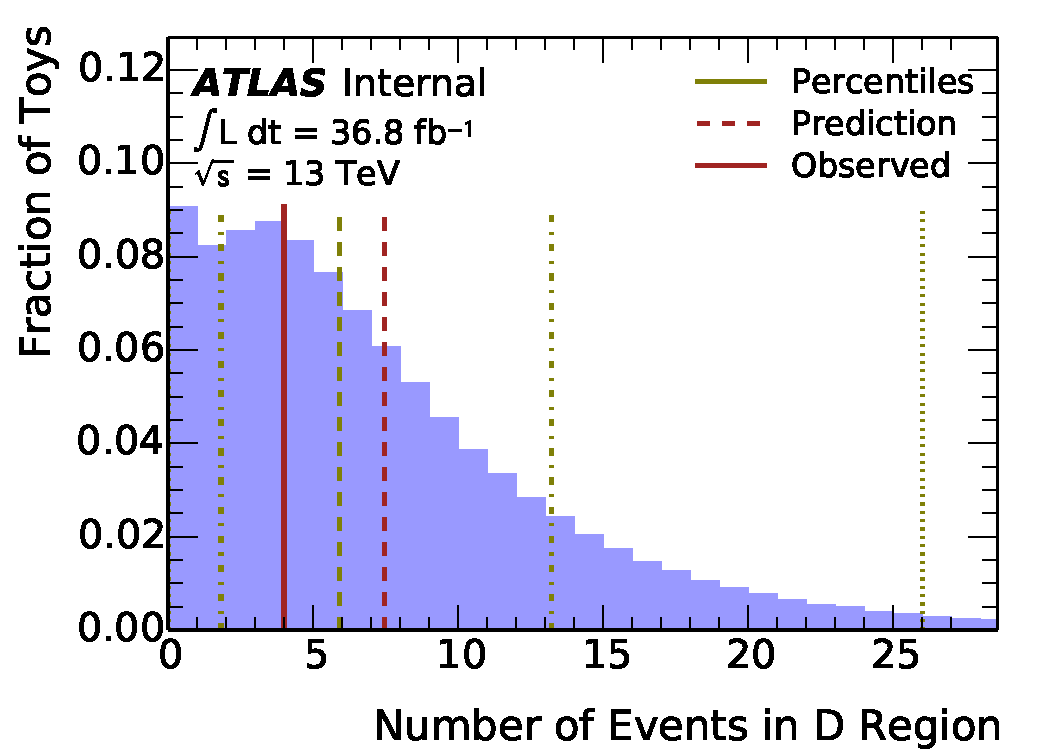
\includegraphics[width=0.45\textwidth]{figures/NinD_distribution_sig_VBF8_m20.pdf}}
  {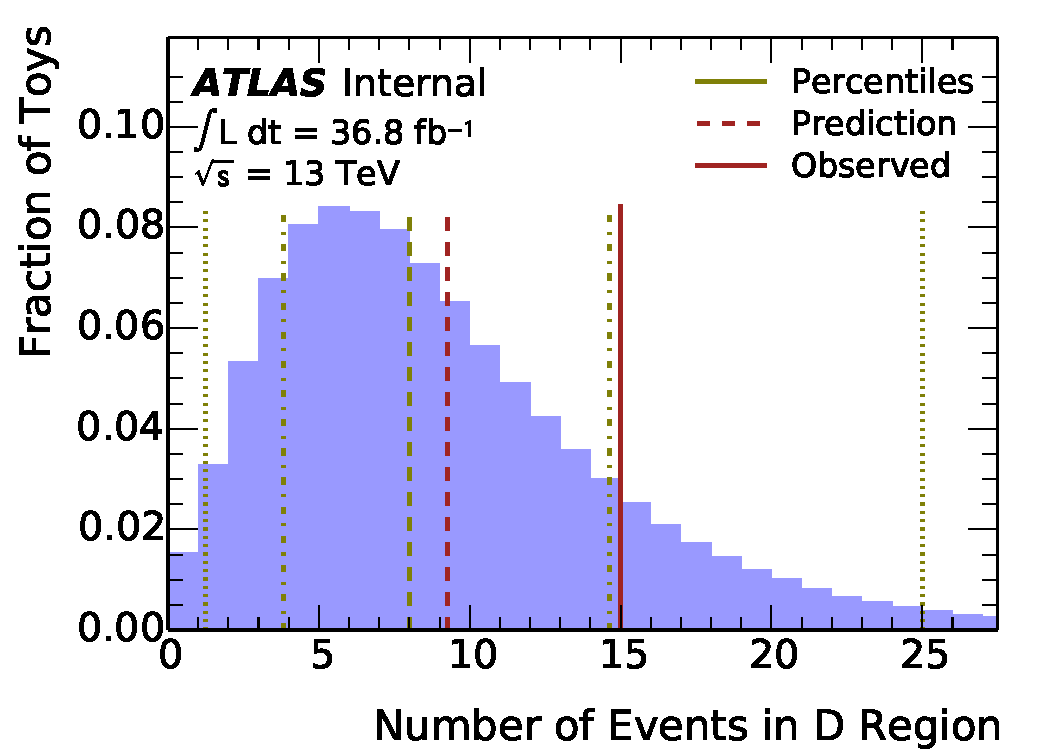
\includegraphics[width=0.45\textwidth]{figures/NinD_distribution_sig_VBF8_m30.pdf}}\\
  {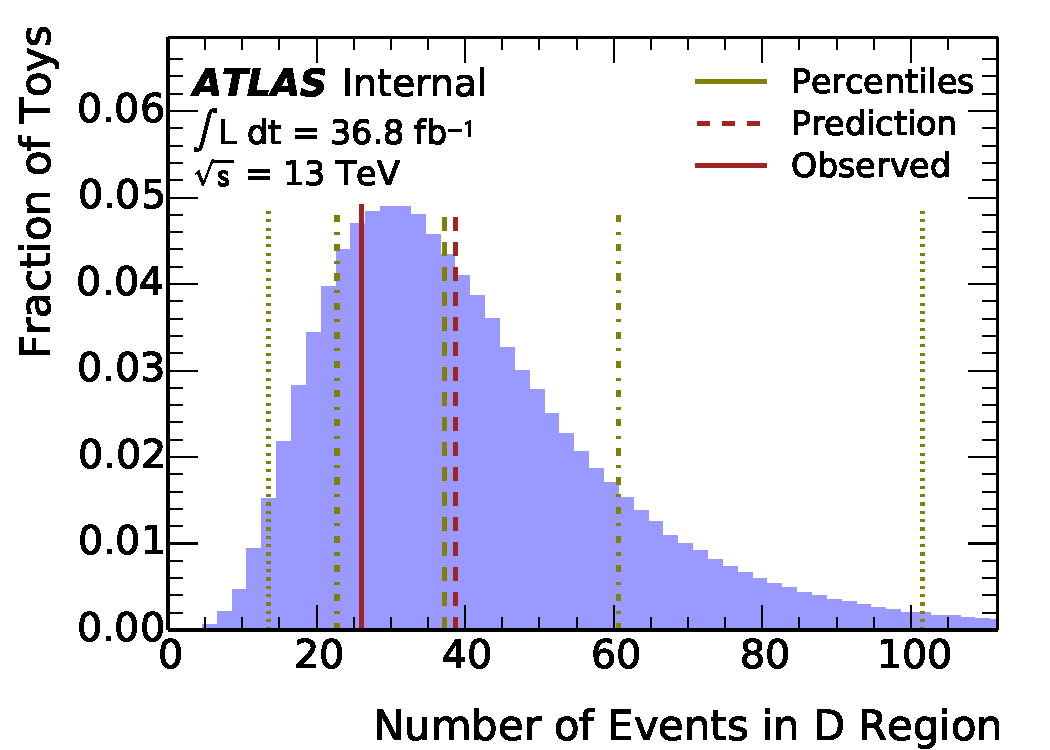
\includegraphics[width=0.45\textwidth]{figures/NinD_distribution_sig_VBF8_m40.pdf}}
  {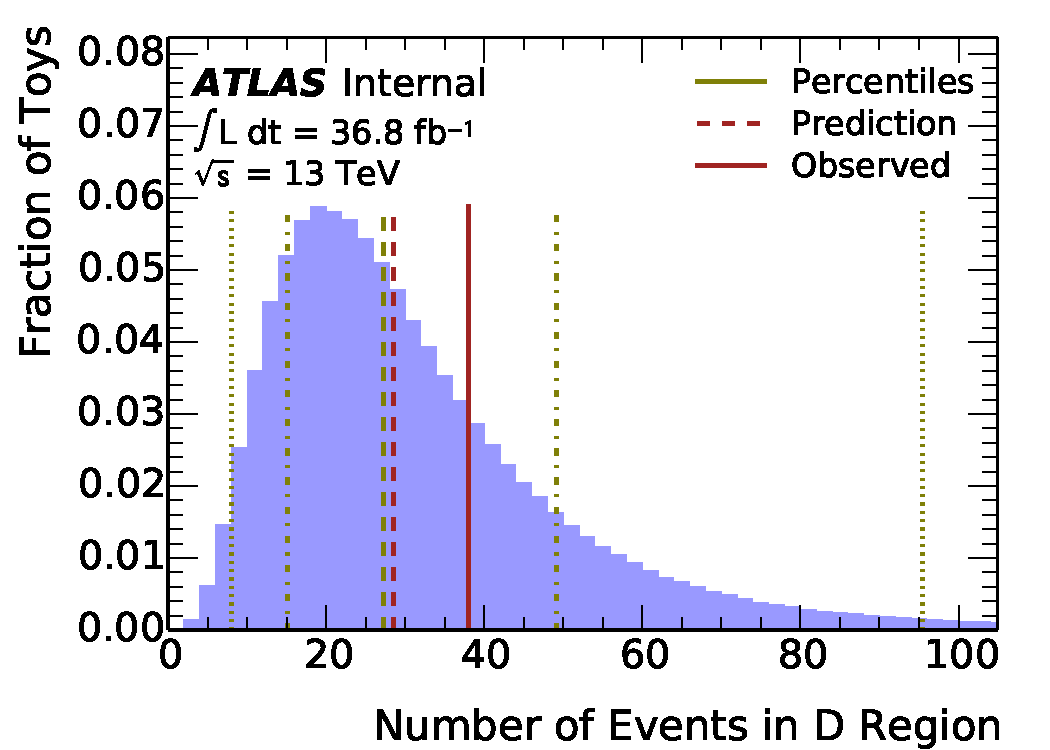
\includegraphics[width=0.45\textwidth]{figures/NinD_distribution_sig_VBF8_m50.pdf}}\\
  {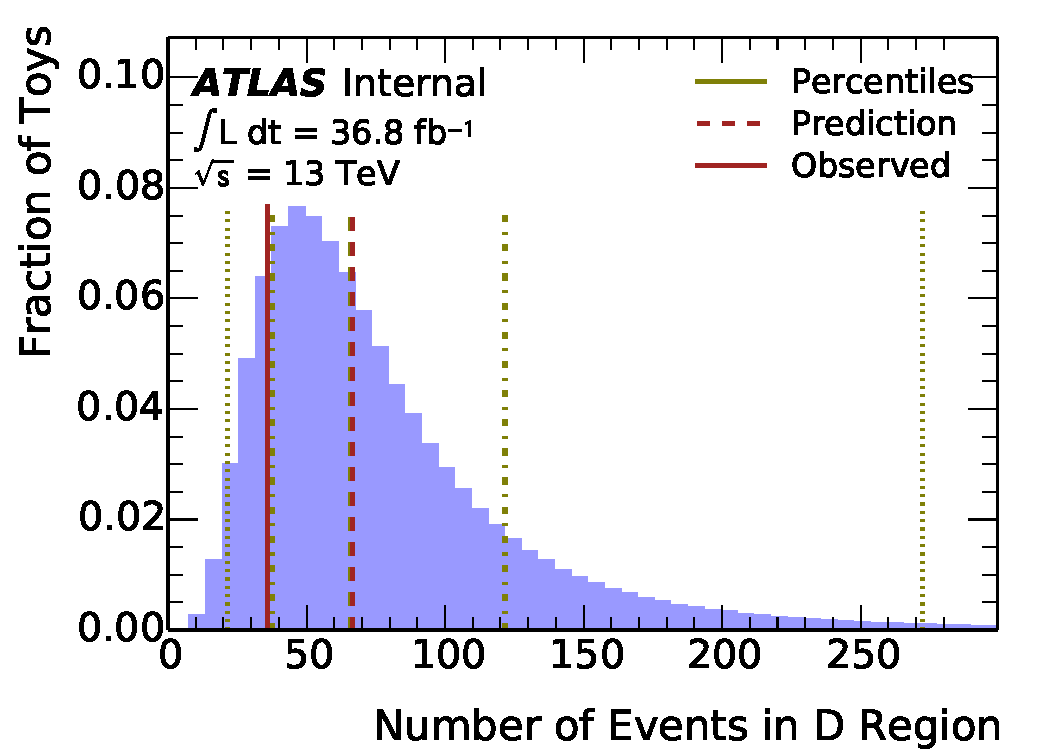
\includegraphics[width=0.45\textwidth]{figures/NinD_distribution_sig_VBF8_m60.pdf}}
  \caption{The blinded prior distribution of possible number of events in the signal $D$ region, taking into account the poisson uncertainty on the control regions $A$, $B$, and $C$.
  The distribution was generated with toys.
In green, the percentiles in the distribution corresponding to the [-2,-1,0,+1,+2]$\sigma$ points of a Normal distribution.
In red, the predicted (dashed) and observed after unblinding (solid) number of events.
(a) Analysis regime 1.
(b) Analysis regime 2.
(c) Analysis regime 3.
(d) Analysis regime 4.
(e) Analysis regime 5.
}
  \label{fig:HBSM:NinD_dist}
\end{figure}
No large excess is observed in region D when comparing the data yield to the background predicted from the A/B/C regions
assuming that the signal is absent in these regions.

\begin{table}[t]
  \begin{center}
    \caption{Number of events observed in each of the A/B/C/D regions, 
      the relative size of the closure uncertainty considered for each $m_{\gamma\gamma}$ regime, 
      and the prediction for the number of background events in region D based on the control region yields.
      The median predicted background yield and its $\pm1\sigma$ uncertainty in region D is also shown.
      The uncertainties in the prediction account for both the Poisson fluctuations of the number of events in the control regions 
      and the closure uncertainty.
    }
    \label{tab:HBSM:ABCD_data}
          {\footnotesize
            \bgroup
            \def\arraystretch{1.3}
	    \begin{tabular}{
                ccccccr@{}l
              }
	      \hline
              $m_{\gamma\gamma}$ regime &   A &   B &   C &   D  & Relative closure uncert. & \multicolumn{2}{c}{Predicted background yield}\\
	      \hline
              1 &  15 &   4 &  28 &   4 &  0.50 & \hspace{1.4cm}6&$^{+7}_{-4}$   \\
              2 &  22 &   6 &  34 &  15 &  0.32 & 8&$^{+7}_{-4}$   \\
              3 &  12 &  16 &  29 &  26 &  0.20 & 37&$^{+23}_{-14}$ \\
              4 &   8 &  12 &  19 &  38 &  0.21 & 27&$^{+22}_{-12}$ \\
              5 &   6 &  20 &  20 &  36 &  0.20 & 66&$^{+56}_{-28}$ \\
	      \hline
	    \end{tabular}
            \egroup
          }
  \end{center}
\end{table}

In order to set limits, the likelihood function (Equation~\ref{eqn:HBSM:likelihood}) is used to fit to all four A/B/C/D regions simultaneously.

The parameter $\mu_\text{S}$ can be expressed as the product of the total integrated luminosity, the signal cross-section 
$\sigma_H\times B(H\to aa\to \gamma\gamma gg)$, and the signal selection efficiency estimated in MC simulation and quoted in Table~\ref{tab:HBSM:ABCD}.

The effects of the uncertainties (Section~\ref{sec:HBSM:statanalysis}) on the estimated number of signal events $\mu_\text{S}$ are studied using Asimov~\cite{Cowan:2010js} pseudo-datasets generated
for an expected signal corresponding to the 95\% CL upper limit obtained in this search (Table~\ref{tab:HBSM:limits}) and using the values of the background 
parameters maximising the likelihood in a fit to data which assumes no signal.
Table~\ref{tab:HBSM:systs} summarises the impact of each source of uncertainty varied by $\pm1\sigma$ on the maximum-likelihood estimate for $\mu_\text{S}$ in each 
of the $m_{\gamma\gamma}$ regimes for an illustrative $m_a$ hypothesis. The statistical uncertainty is the largest one for all regimes.
\begin{table}[t]
  \begin{center}
    \caption{
      Maximum fractional impact on the fitted $\mu_\text{S}$ from sources of systematic uncertainty estimated using Asimov datasets.
      The signal injected in the Asimov datasets corresponds to the observed upper limit quoted in Table~\ref{tab:HBSM:limits}.
    }
    \label{tab:HBSM:systs}
          {\footnotesize
	  \begin{tabular}{cccccc}
	  \hline
          &\multicolumn{5}{c}{$m_{\gamma\gamma}$ regime} \\
          Source of Uncert.   &    1  &   2  &   3  &   4  &   5  \\
            &   $m_a=20~\GeV{}$ &  $m_a=30~\GeV{}$ &  $m_a=40~\GeV{}$ &  $m_a=50~\GeV{}$ &  $m_a=60~\GeV{}$ \\
          \hline
	  Statistical          &     0.73 &     0.51 &     0.89 &     1.13 &     0.92 \\
	  Closure              &     0.44 &     0.27 &     0.39 &     0.64 &     0.89 \\
	  \hline
	  Modelling            &     0.35 &     0.34 &     0.46 &     0.42 &     0.65 \\
	  Jet                  &     0.58 &     0.38 &     0.25 &     0.90 &     0.71 \\
	  Photon               &     0.06 &     0.05 &     0.10 &     0.12 &     0.13 \\
	  Lumi and Pile-up     &     0.06 &     0.04 &     0.27 &     0.14 &     0.32 \\
	  \hline
	  \end{tabular}
          }
  \end{center}
\end{table}

The best-fit values of the parameters of the likelihood function are given in Table~\ref{tab:HBSM:MLE}.
The probability that the data are compatible with the background-only hypothesis is computed for each $m_{\gamma\gamma}$ regime and no significant 
excess is observed. The smallest local $p$-value, obtained for the $m_{\gamma\gamma}$ regime 2 ($m_a\approx30~\GeV{}$), is of the order of 4\%.
\begin{table}[t]
  \begin{center}
    \caption{Maximum-likelihood fit values for each of the free parameters of the likelihood function 
      in each $m_{\gamma\gamma}$ regime for a relevant signal $m_a$ hypothesis.
      The estimated uncertainties in the fit parameters assume
      that the likelihood function is parabolic around the minimum of the fit.
    }
    \label{tab:HBSM:MLE}
          {\footnotesize
	    \begin{tabular}{
                cc
                r@{}lr@{}l
                r@{}lr@{}l
              }
	      \hline
              $m_{\gamma\gamma}$ regime & $m_a$ [\GeV{}] &   \multicolumn{2}{c}{$\mu_\text{S}$} &   \multicolumn{2}{c}{$\mu_\text{bkg}$}  &   \multicolumn{2}{c}{$\tau_\text{B}$} & \multicolumn{2}{c}{$\tau_\text{C}$} \\
	      \hline
              1 & 20 &  -7&$\pm$18    & 11&$\pm$17   & 0.5 &$\pm$0.4 &  2.9&$\pm$3.1   \\
              2 & 30 &  8&$\pm$8      & 7&$\pm$6     & 0.68 &$\pm$0.32 & 4.3&$\pm$3.1   \\
              3 & 40 &  -30&$\pm$80   & 60&$\pm$70   & 0.35 &$\pm$0.19 & 0.67&$\pm$0.33 \\
              4 & 50 &  22&$\pm$28    & 16&$\pm$23   & 0.5 &$\pm$0.4 & 0.9&$\pm$1.0   \\
              5 & 60 &  -290&$\pm$260 & 340&$\pm$340 & 0.21&$\pm$0.05 & 0.24&$\pm$0.05 \\
	      \hline
	    \end{tabular}
          }
  \end{center}
\end{table}
Since no significant excess is observed, an upper limit is derived at 95\% CL.            
The expected and observed exclusion limits on $\mu_\text{S}$ are given in Table~\ref{tab:HBSM:limits}.
This is related to the limit on the $pp\to H\to aa \to \gamma\gamma gg$ cross-section by appropriately normalising to the measured total integrated luminosity 
and selection efficiencies relative to the inclusive signal production obtained from the ggF and VBF MC samples (Table~\ref{tab:HBSM:ABCD}).
The limit is also expressed relative to the SM cross-section for the Higgs boson, shown in Figure~\ref{fig:HBSM:brazil_ma}.
Within a $m_{\gamma\gamma}$ analysis regime, limits are interpolated linearly in between simulated $m_a$ values.
Finally, for each mass point, the $m_{\gamma\gamma}$ regime that yields the best expected limit is used to provide the observed exclusion limit.
The limit is calculated using a frequentist $\text{CL}_\text{s}$ calculation~\cite{Read:2002hq}. 

\begin{table}[t]
  \begin{center}
    \caption{Observed (expected) upper limits at the 95\% CL, for each of the $m_a$ values considered in the search.
      In each case, the $m_{\gamma\gamma}$ regime used to calculate the limits is also indicated.
      The uncertainties include both the statistical and systematic sources of uncertainty in the fit.}
    \label{tab:HBSM:limits}
          {\footnotesize
            \bgroup
            \def\arraystretch{1.5}
            \begin{tabular}{ccr@{}lr@{}lr@{}l}
	    \hline
            $m_{\gamma\gamma}$ regime & $m_a$ [\GeV{}] & \multicolumn{2}{c}{$\mu_\text{S}$}   & \multicolumn{2}{c}{$\sigma_H\times B(H\to aa \to \gamma\gamma gg)$ [pb]}  & \multicolumn{2}{c}{$\frac{\sigma_H}{\sigma_\text{SM}}\times B(H\to aa \to \gamma\gamma gg)$} \\
	    \hline
            1 & 20 & $10.8\Big(10.4$&$^{+4.6}_{-3.1}\Big)$   & \hspace{1.1cm}$4.8\Big(4.6$&$^{+2.1}_{-1.4}\Big)$  & \hspace{0.505cm}$0.086\Big(0.082$&$^{+0.037}_{-0.025}\Big)$ \\
            1 & 25 & $10.4\Big(10.9$&$^{+3.8}_{-2.5}\Big)$   & $1.9\Big(2.0$&$^{+0.7}_{-0.5}\Big)$  & $0.034\Big(0.036$&$^{+0.013}_{-0.008}\Big)$ \\
            2 & 25 & $28\Big(25$&$^{+8}_{-6}\Big)$   & $5.1\Big(4.7$&$^{+1.4}_{-1.1}\Big)$  & $0.092\Big(0.084$&$^{+0.026}_{-0.019}\Big)$ \\
            2 & 30 & $29\Big(24$&$^{+11}_{-6}\Big)$  & $3.1\Big(2.6$&$^{+1.1}_{-0.7}\Big)$ & $0.056\Big(0.046$&$^{+0.021}_{-0.012}\Big)$ \\
            2 & 35 & $27\Big(22$&$^{+9}_{-6}\Big)$   & $2.7\Big(2.2$&$^{+0.9}_{-0.6}\Big)$ & $0.049\Big(0.040$&$^{+0.016}_{-0.011}\Big)$  \\
            3 & 35 & $30\Big(36$&$^{+18}_{-9}\Big)$  & $2.7\Big(3.2$&$^{+1.6}_{-0.8}\Big)$ & $0.048\Big(0.057$&$^{+0.028}_{-0.014}\Big)$  \\
            3 & 40 & $31\Big(39$&$^{+19}_{-12}\Big)$ & $3.2\Big(4.0$&$^{+2.0}_{-1.2}\Big)$  & $0.058\Big(0.073$&$^{+0.035}_{-0.022}\Big)$ \\
            3 & 45 & $45\Big(53$&$^{+15}_{-20}\Big)$ & $6.3\Big(7.5$&$^{+2.1}_{-2.8}\Big)$   & $0.113\Big(0.134$&$^{+0.038}_{-0.050}\Big)$     \\
            4 & 45 & $74\Big(68$&$^{+16}_{-15}\Big)$ & $9.2\Big(8.4$&$^{+2.0}_{-1.9}\Big)$  & $0.166\Big(0.152$&$^{+0.036}_{-0.034}\Big)$ \\
            4 & 50 & $79\Big(77$&$^{+17}_{-16}\Big)$ & $9.0\Big(8.8$&$^{+2.0}_{-1.8}\Big)$  & $0.162\Big(0.159$&$^{+0.036}_{-0.032}\Big)$   \\
            4 & 55 & $73\Big(69$&$^{+11}_{-10}\Big)$  & $9.7\Big(9.1$&$^{+1.5}_{-1.2}\Big)$   & $0.173\Big(0.163$&$^{+0.026}_{-0.022}\Big)$    \\
            5 & 55 & $48\Big(59$&$^{+41}_{-19}\Big)$ & $5.5\Big(6.8$&$^{+4.7}_{-2.1}\Big)$  & $0.10\Big(0.12$&$^{+0.08}_{-0.04}\Big)$ \\
            5 & 60 & $67\Big(81$&$^{+24}_{-31}\Big)$ & $8.0\Big(9.5$&$^{+2.8}_{-3.6}\Big)$  & $0.14\Big(0.17$&$^{+0.05}_{-0.07}\Big)$   \\
	    \hline
	    \end{tabular}
            \egroup
          }
  \end{center}
\end{table}

\begin{figure}[t]
  \centering 
  {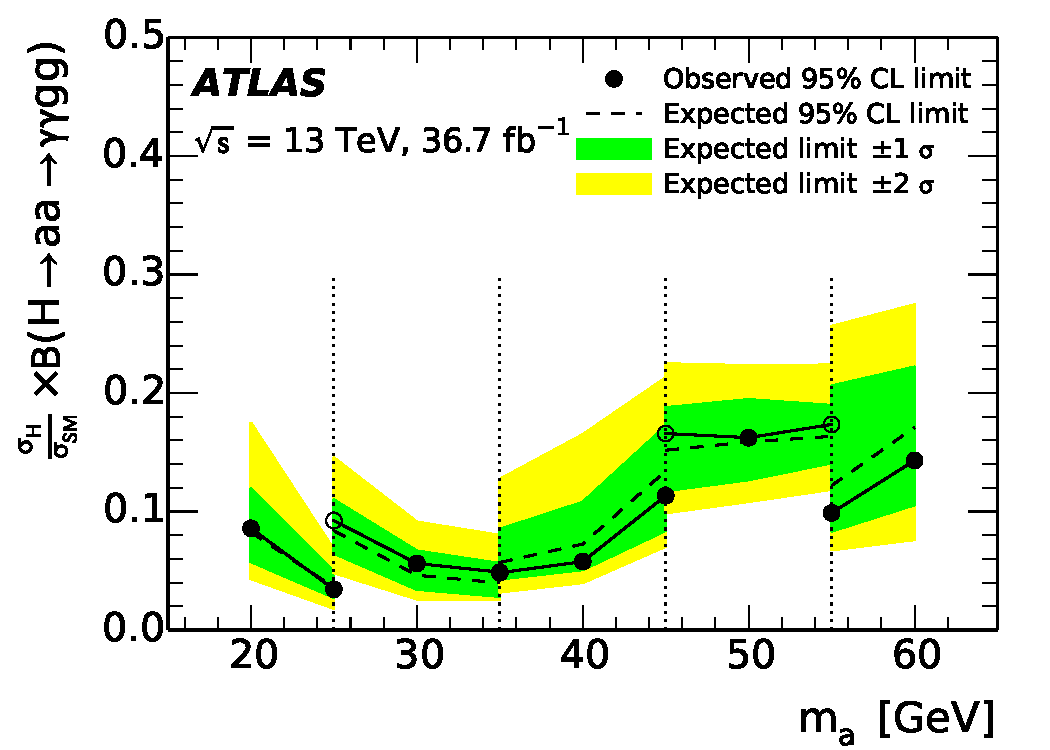
\includegraphics[width=0.9\textwidth]{figures/ABCD_twosigma_brazil_Freq_systs_obs_HF_ma_2_16_18.pdf}}
  \caption{The observed (solid line) and expected (dashed line) 95\% CL exclusion upper limit on 
    the \mbox{$pp\to H\to aa \to \gamma\gamma gg$} cross-section times branching ratio as a function of $m_a$,
    normalised to the SM inclusive $pp\to H$ cross-section~\cite{deFlorian:2016spz}.
  The vertical lines indicate the boundaries between the different $m_{\gamma\gamma}$ analysis regimes.
  At the boundaries, the $m_{\gamma\gamma}$ regime that yields the best expected limit is used to provide the observed exclusion limit (filled circles); the observed limit provided by the regime that yields the worse limit is also indicated (empty circles).
}
  \label{fig:HBSM:brazil_ma}
\end{figure}

\clearpage
\section{Discussion}
This analysis can be combined with the Run 1 search for $H\to 2a \to 4\gamma$~\cite{Aad:2015bua}
to place a limit on the overall BR$(H\rightarrow aa)$. 
Figure~\ref{fig:HBSM:compare_4gamma} shows a quantitative comparison of the two analyses.

The two analyses have different sensitivities in different parts of the phase space, 
parameterized by $\rho=\text{BR}(a\rightarrow \gamma\gamma)/\text{BR}(a\rightarrow jj)$. 
The analysis presented in this note is more sensitive for lower values of $\rho$, 
closer to SM-like couplings with photons and gluons; a typical value of $\rho$ in a 2HDM model as discussed in~\cite{Curtin:2013fra} is shown for reference.
The $H\to 2a \to 4\gamma$ search is more sensitive if there is a large BR to photons.
 
Both of these analyses are limited by statistics, 
therefore these bounds will improve with more data. 

\begin{figure}[htbp]
  \centering 
  \subfloat[]{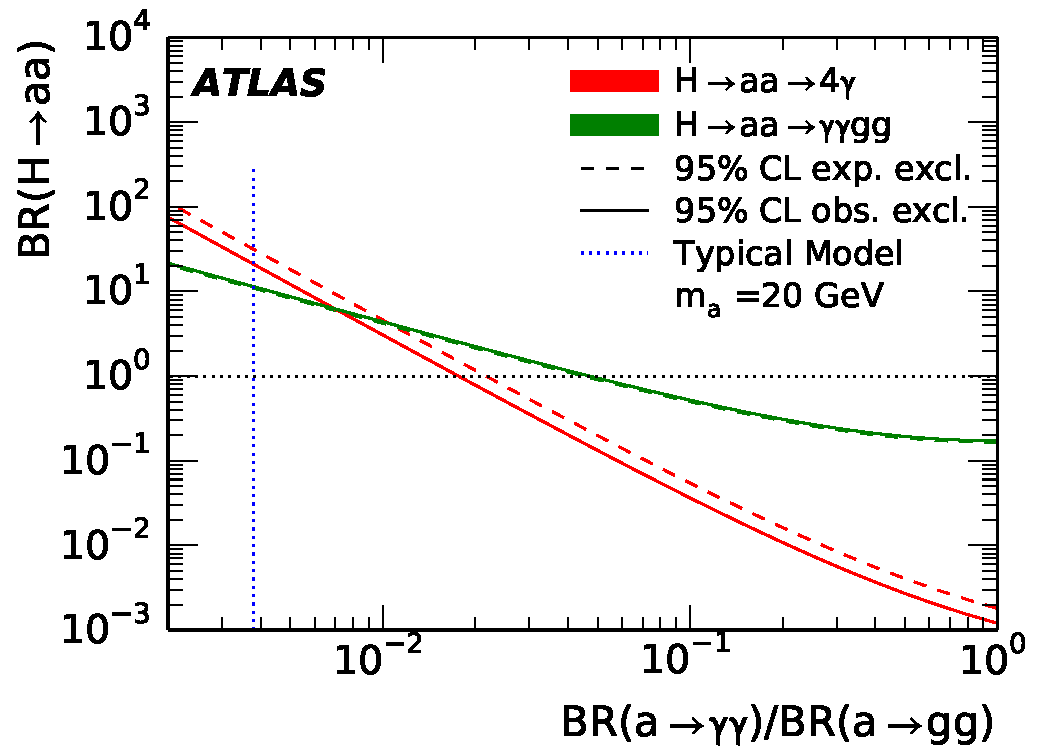
\includegraphics[width=0.45\textwidth]{figures/compare_4gamma_20.pdf}}
  \subfloat[]{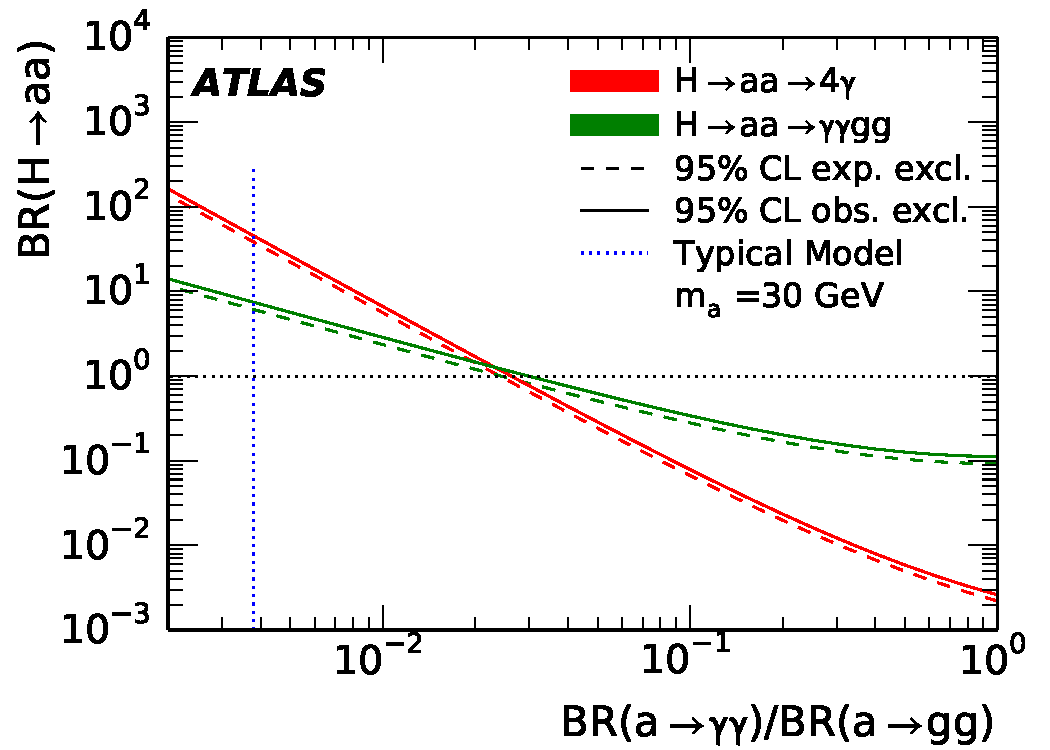
\includegraphics[width=0.45\textwidth]{figures/compare_4gamma_30.pdf}}\\
  \subfloat[]{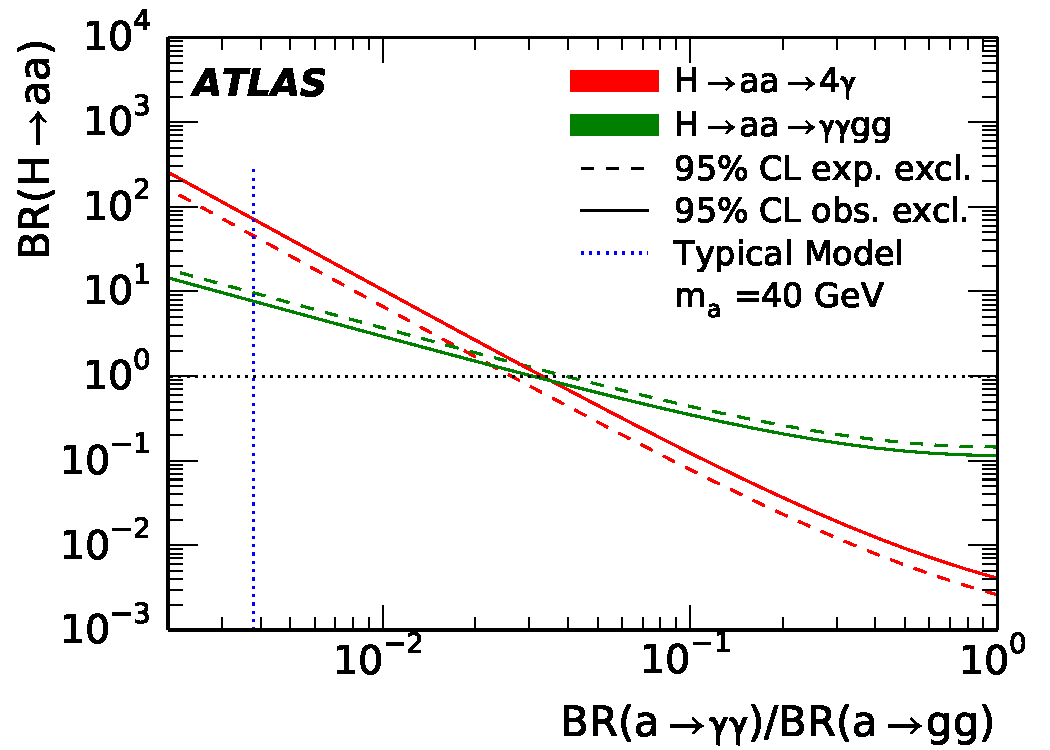
\includegraphics[width=0.45\textwidth]{figures/compare_4gamma_40.pdf}}
  \subfloat[]{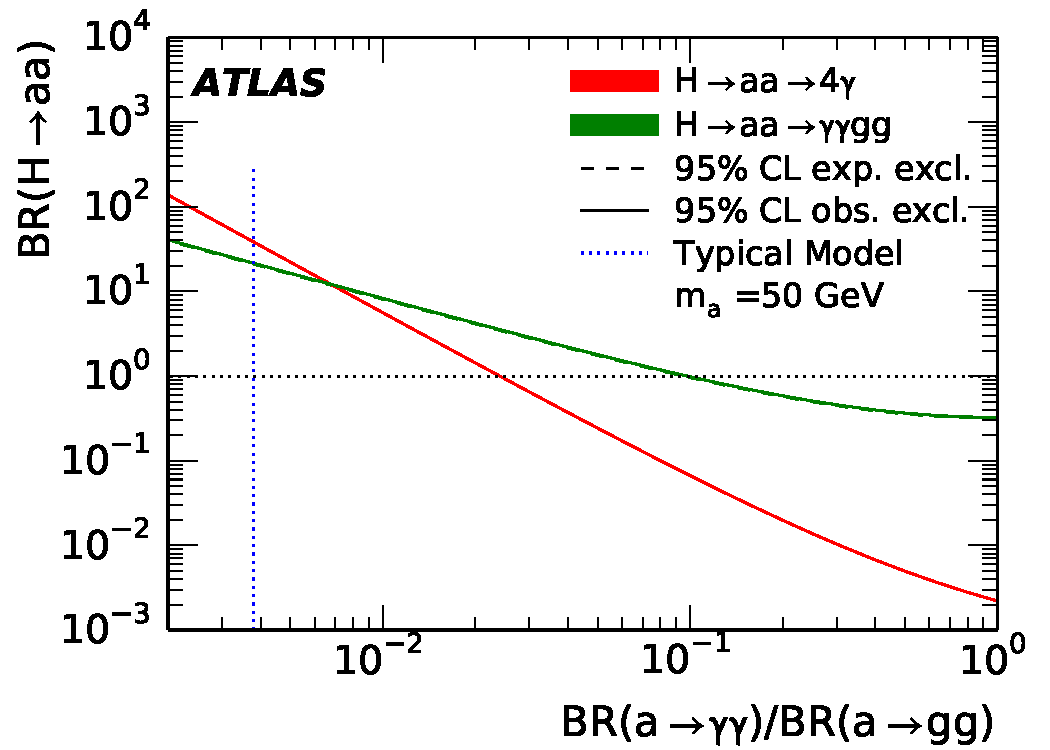
\includegraphics[width=0.45\textwidth]{figures/compare_4gamma_50.pdf}}\\
  \subfloat[]{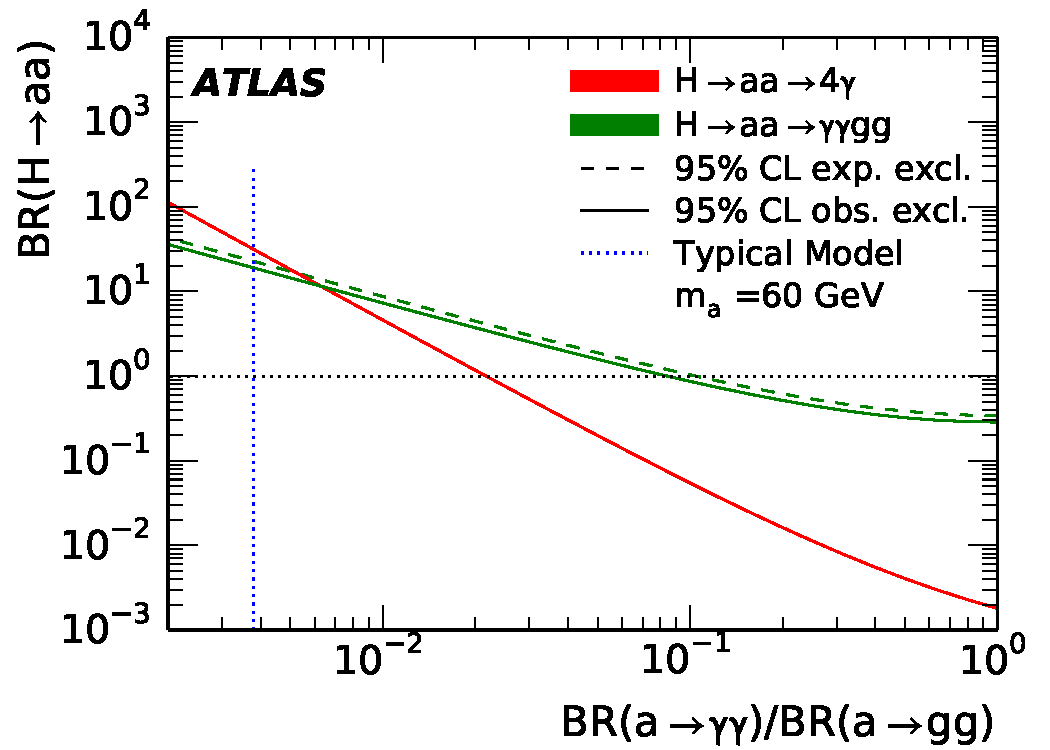
\includegraphics[width=0.45\textwidth]{figures/compare_4gamma_60.pdf}}
  \caption{The exclusion limit placed on BR$(H\rightarrow aa)$ as a function of BR$(a\rightarrow \gamma\gamma)/\text{BR}(a\rightarrow jj)$, and comparing the ATLAS 4$\gamma$ analysis to this analysis. Also shown is a typical value for BR$(a\rightarrow \gamma\gamma)/\text{BR}(a\rightarrow jj)$ in the NMSSM. (a) $m_a=$20 GeV. (b) $m_a=$30 GeV. (c) $m_a=$40 GeV. (d) $m_a=$50 GeV. (e) $m_a=$60 GeV.}
  \label{fig:HBSM:compare_4gamma}
\end{figure}

This search is notably limited to $m_a\ge20$ \GeV{}; the ATLAS Run 1 search for $H\rightarrow aa \to 4\gamma$~\cite{Aad:2015bua} similarly sets limits only for $m_a\ge10$ \GeV{}.
As mentioned in Section~\ref{sec:HBSM:trigger} and Section~\ref{sec:HBSM:photons}, these lower bounds are due to the limitations set by using the diphoton trigger and the diphoton selection.
For low $m_a$, the $a$ particle is boosted and the decay products are collimated - this ruins the efficiency of the diphoton selection, both because of the way photon objects are constructed in the calorimeter at trigger level and because isolation is imposed on the photons in the offline object reconstruction.
This inefficiency is discussed in detail in Appendix~\ref{ch:HBSM_lowmass_app}.
Thus, new techniques will be required to set limits on lower masses.

Reference~\cite{Aaboud:2018djx} demonstrates a search for $X\rightarrow aa\rightarrow 4\gamma$ with $X$ a high-mass scalar particle with mass between $200$ and $2000$ \GeV{} (notably missing the Higgs mass $m_H\sim 125$ \GeV{}) and $a$ with mass between $100$ MeV and up to between $2$ and $10$ \GeV{}, depending on the $X$ mass.
There is a similar search~\cite{ATLAS-CONF-2012-079} from Run 1 that sets limits for $X$ with a mass between $110$ and $150$ \GeV{} and $m_a$ between 100 and 400 MeV.
These searches are accomplished by taking advantage of the fact that in these regimes, the $a$ is highly boosted, so that the photon decay products end up collimated in a single photonlike energy cluster and the trigger identiies these as a single isolated photon.
Substructure of this photonlike energy cluster is used offline to enhance the signal presence.

Appendix~\ref{ch:HBSM_lowmass_app} proposes an already existing trigger and offline selection strategy that can be sensitive to $H\rightarrow aa\rightarrow gg\gamma\gamma$ with $m_a<20$ \GeV{}, and could enable a search for these low masses.
Though not necessary to enable this search, the weak supervision analysis techniques used in Chapter~\ref{ch:CWoLa} could be used to search for these signals while retaining limited dependence on the background simulation.


This search also presents many interesting areas of research in order to improve the sensitivity of the analysis for the resolved mass range $m_a\ge 20$ \GeV{}.
The event selection (Section~\ref{sec:HBSM:jets}) requires four jets, and this analysis is enabled by the use of these jets, in keeping with the overall theme of this Thesis.
The main challenges present in the analysis include the correct identification of the VBF and signal jets; the VBF selection including the VBF $m_{jj}$ selection and the leading VBF jet \pt{}; the resolution of the signal jet $m_{jj}$, which directly affects the resolution of $|m_{jj}-m_{\gamma\gamma}|$; and the final resolution of the signal $m_{jj\gamma\gamma}$.

The identification of the VBF and signal jets could be aided by using techniques intended to discriminate between jets initiated by quarks and those initiated by gluons~\cite{ATL-PHYS-PUB-2017-009,Aad:2014gea,ATLAS-CONF-2016-034,ATL-PHYS-PUB-2017-017}.

Each of the remaining challenges would be better tackled by improving the energy and \pt{} resolution of the jets involved, since the invariant mass is a simple function of the individual jet energies and the angle between them\footnote{Actually, this would help with all the challenges mentioned, since the VBF selection also relies on the resolution of the VBF $m_{jj}$.}.
When reconstructing the true energy of a jet, both the effects of the energy response of the calorimeter and the effect of other proton-proton interactions in the event (pile-up) must be taken into account.
Chapter~\ref{ch:NI} presents work on studying in a rigorous framework the mathematical process of reversing the effects of the calorimeter response in order to access the originating parton energy~\cite{Cukierman:2016dkb};
and Chapter~\ref{ch:GenNI} presents work on using machine learning to further improve this process~\cite{ATL-PHYS-PUB-2018-013}.
%Appendix~\ref{ch:Voronoi} presents work on novel jet reconstruction algorithms which aim to reduce the effect of pileup on the jet reconstructed energy~\cite{ATLAS-CONF-2017-065}.
The Author has also worked on novel jet reconstruction algorithms which aim to reduce the effect of pileup on the jet reconstructed energy~\cite{ATLAS-CONF-2017-065}.
By better reconstructing the energies of the jets that appear in the final state of this analysis, these efforts can improve the ultimate sensitivity of this search, in addition to being broadly applicable to other analyses than the one being studied here. 

\clearpage
\section{Conclusion}
\label{sec:HBSM:conclusion}
In summary, a search for exotic decays of the Higgs boson into a pair of new (pseudo)scalar particles,
$H\to aa$, in final states with two photons 
and two jets is conducted using 36.7~\ifb{} of $pp$ collisions at $\sqrt{s}=13$ \TeV{} recorded 
with the ATLAS detector at the LHC. The search for $H\to aa \to \gamma\gamma gg$ is performed
in the mass range $20 < m_a < 60~\GeV{}$ and with additional jet requirements 
to enhance VBF-produced signal while suppressing the $\gamma\gamma$+jets background.
No significant excess of data is observed relative to the SM predictions. An upper limit
is set for the product of the production cross-section for $pp\to H$ and the branching
ratio for the decay $H\to aa\to\gamma\gamma gg$. The upper limit ranges from 3.1 pb to 9.0 pb depending
on $m_a$, and is mostly driven by the statistical uncertainties.
These results complement the previous upper limit on $H\to aa\to\gamma\gamma\gamma\gamma$ and
further constrains the BSM parameter space for exotic decays of the Higgs boson.

This search can be extended to the low-mass regime using novel techniques (Appendix~\ref{ch:HBSM_lowmass_app}).
In particular, the weak supervision analysis techniques used in Chapter~\ref{ch:CWoLa} could be used to target this low-mass regime.
The sensitivity of the search presented here, and the extension to the low-mass regime, can be improved utilizing the novel technique for jet calibrations proposed in Chapter~\ref{ch:GenNI}, which builds upon the deep understanding of calibrations provided in Chapter~\ref{ch:NI}.
